\documentclass[12pt,a4paper]{report}
\usepackage[utf8]{inputenc}
%\usepackage[default,regular,bold]{sourceserifpro} % définition de la police à utiliser dans le pdf. ref : http://www.tug.dk/FontCatalogue/sourceserifprolight/

%\usepackage{gfsartemisia}
\usepackage{mathpazo}
\usepackage[scaled=0.95]{helvet}
\usepackage{courier}
\usepackage[T1]{fontenc}
\usepackage{amsmath,amsfonts,amssymb}

\usepackage{setspace} %package pour l'interligne

\usepackage[francais, english]{babel} 

\AddThinSpaceBeforeFootnotes % à insérer si on utilise \usepackage[french]{babel}
\FrenchFootnotes % à insérer si on utilise \usepackage[french]{babel}

\usepackage[top=3cm, bottom=3cm, left=3cm, right=3cm]{geometry} % définition des marges
\usepackage{hyperref} %pour rendre la table des matières cliquable a l'intérieur du document
\usepackage{fancyhdr} %package pour les entetes et les pieds de page , voir http://www.xm1math.net/doculatex/entetepied.html

\usepackage{shorttoc} %ce  package permet de générer un sommaire

\usepackage{minted}% package pour la coloration de code dans latex
\usemintedstyle{manni}

\usepackage{graphicx}

\usepackage{pdfpages} 

\pagestyle{fancy} % définition du style des entetes et pied de page
\renewcommand{\headrulewidth}{1pt}
%\fancyhead[C]{\textbf{page \thepage}} 
%\fancyhead[L]{\thesection}
\fancyhead[R]{\small}

\renewcommand{\footrulewidth}{0pt}
\fancyfoot[C]{\textbf{ \thepage}} 
%\fancyfoot[L]{truc}
%\fancyfoot[R]{\leftmark}

%pour les tableaux
\usepackage{array,multirow,makecell}
\setcellgapes{1pt}
\makegapedcells
\newcolumntype{R}[1]{>{\raggedleft\arraybackslash }b{#1}}
\newcolumntype{L}[1]{>{\raggedright\arraybackslash }b{#1}}
\newcolumntype{C}[1]{>{\centering\arraybackslash }b{#1}}


\author{Bamouni Kevin}
\title{Détection d'anomalies par isolation et missions transversales}

\onehalfspacing % définition d'un interligne 1.5 pour tout le document

\begin{document}

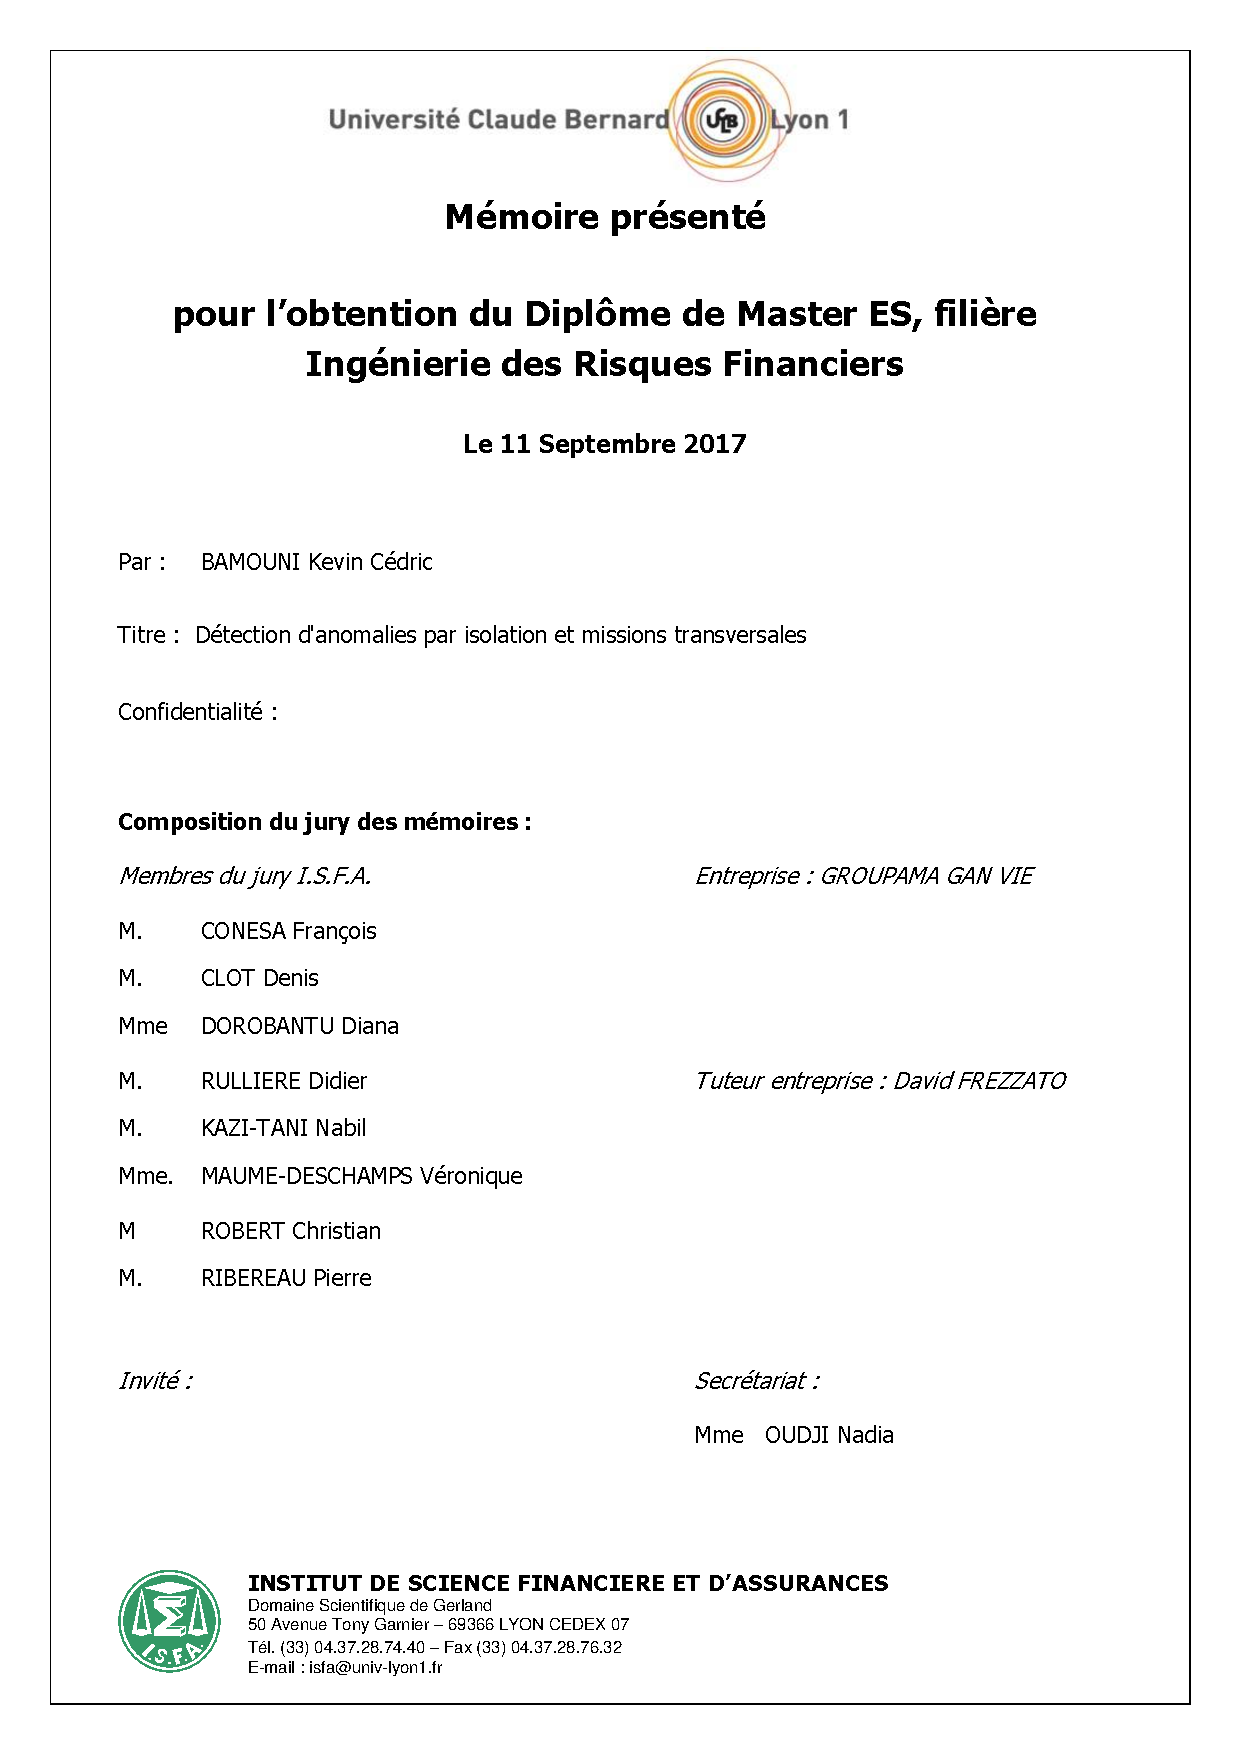
\includepdf[pages=-]{couverture.pdf}

\maketitle

\input{titres/titre.tex}

\input{titres/garde.tex}

\pagenumbering{roman} % on lui informe que les chiffres à utiliser sont les romains
\setcounter{page}{1} % commence à numéroter à partir de 1

\addcontentsline{toc}{chapter}{Résumé}
\chapter*{Résumé} 

\begin{singlespace}
\textbf{Mots clés~:} python, apprentissage, automatique, machine learning, isolation, anomalie, distribution.
\end{singlespace}

Les équipes techniques au sein de sociétés d'assurances utilisent tout un ensemble d'outils et de méthodes pour accomplir des tâches simples et complexes. Dans un contexte d'évolution dynamique, ces outils et méthodes ont tout aussi besoin d'évoluer. C'est dans ce contexte que python et l'apprentissage automatique arrivent en assurance vie, pour apporter de la performance de l'efficacité et de l'innovation. 
\\
\\
Ce rapport a pour objectif de présenter l'ensemble des missions transverses qui ont pu être exécutées avec python. Il montre comment python se veut un outil, utile et puissant. Python n'est plus un simple langage de programmation, il devient un sérieux concurrent de SAS en terme de manipulation et de d'analyse de données. En outre, il a aussi permit de construire un modèle de détection d'anomalies, basé sur le concept de machine learning, pour la fiabilisation de données. Python dispose d'une multitude de bibliothèques qui font de lui, un langage complet.



\addcontentsline{toc}{chapter}{Abstract}
\chapter*{Abstract}
\selectlanguage{english}

In insurance companies, technical teams use a set of tools to achieve all kind of missions and take up challenges continuously. In a dynamic world, insurrance and finance are always facing new problems, so they need to improve new technics and tools. That way, python and machine learning came in life insurance. 
\\
\\
This report aim to present all the missions i accomplished during my intern in Groupama Gan Vie with python as my main tool. It shows how python is a very useful and powerful programming language. Python is a whole set of tools in itself. It can do data analysis, manipulation, and machine learning. I also participate in the elaboration of an anomaly detection model for the assets and liabilities management practice. This model is essentially to make data reliable.

\begin{singlespace}
\textbf {Keywords ~:} python, machine, learning, isolation, anomaly, distribution.
\end{singlespace}

\selectlanguage{french}

\addcontentsline{toc}{chapter}{Remerciements}
\chapter*{Remerciements} 

Je remercie David FREZZATO de m'avoir permis d'effectuer cet alternance à ses côtés, pour sa disponibilité et son assistance en continue.  	
\\
\\
Je remercie l'ensemble de l'équipe de l’actuariat de m'avoir intégré et accompagné.
\\
\\
Je remercie Diana DOROBANTU et Denis CLOS pour l'ensemble de leurs efforts continues pour la réussite des étudiants du master d'ingénierie des risques.

% le sommaire, il est moins détaillé que la table des matières
\selectlanguage{french}
%\renewcommand{\contentsname}{Sommaire} %permet de changer le titre table des matières en sommaire dans le document
%\setcounter{tocdepth}{1} %defini la profondeur maximale des titres du sommaire
%\tableofcontents % Sommire en debut et/ou table des matières en fin de rapport
{\setlength{\baselineskip}{0.9\baselineskip}
\shorttableofcontents{Sommaire}{1}
\par}


\pagenumbering{arabic} % fin numérotation en chiffres romains, % début numérotation en chiffres arabs3
\setcounter{page}{1} 

% Introduction
\addcontentsline{toc}{chapter}{Introduction}
\chapter*{Introduction}
Au cours de ma deuxième année de master en ingénierie des risques financiers, j'ai occupé un poste de chargé d'études actuarielles à GROUPAMA GAN VIE. J'ai travaillé sur des missions dans des domaines variés.
\\
\\
Ce document se présente en deux parties. Un rapport dans lequel j'aborde l'ensemble des grandes missions que j'ai eu à effectuer. Pour chaque mission j'aborde la problématique, l'exécution et les éventuelles difficultés rencontrées.
\\
\\
L'ensemble des travaux effectués, ont pour principal objectif de faciliter et fiabiliser les différents processus avec des outils fiables et simples. En effet, certains outils se montrent de moins en moins pratiques. J'ai passé ainsi une bonne partie de mon alternance à construire, implémenter et tester de nouveaux outils avec le langage de programmation python comme meilleur compagnon.
\\
\\
La seconde partie est consacrée à l'étude d'un article scientifique qui présente une méthode de machine learning de la bibliothèque scikitlearn de python. Cette méthode à été utilisée pour la création d'un modèle qui permettra la détection d'anomalies dans un ensemble de données.





\part{Rapport d'alternance}
\label{prt:missions} % utilisé pour faire des références dans le texte, pas besoin d'écrire le nom ou le numéro de la partie on donne juste le nom et lui il se charge de le remplacer par le nom

%\chapter{GROUPAMA GAN VIE (GGVie)}
GROUPAMA GAN VIE \footnote{ Description disponible sur http://www.groupama.com/fr/fiche/groupama-gan-vie/} (GGVie) est la société vie unique du groupe GROUPAMA. Elle assure la conception, la souscription et la gestion des contrats d'assurances de personnes (épargne, retraite, prévoyance et santé) commercialisés par les cinq réseaux de distribution du Groupe (les Caisses régionales, Gan Assurances, Gan Patrimoine, Gan Prévoyance et le courtage). Elle est organisée autour de deux directions métiers - Individuelle et Collective - et de trois directions fonctionnelles (Affaires générales et risque management, Financière, Ressources Humaines et Communication interne).

Mon alternance s'est déroulé au sein du service de veille réglementaire et technologique (SVRT). Sous la direction financiére, le service veille essentiellement à l'application des différentes normes auxquelles est soumise la société. Ses principales missions sont :
\begin{itemize}
\item S'assurer du respect des processus de calcul et des quantités règlementaires.
\item De la gestion actif passif dans un contexte ORSA (Own Risk and Solvency Assessment) de Solvabilité \textsc{II}
\item Des reporting réglementaires \textsc{II}.
\item De la recherche et de la promotion de nouveaux outils open source.
\end{itemize}

En tant que chargé d'études actuarielles au sein du service, j'étais en charge de la veille technologique. j'avais pour mission de trouver des nouveaux outils et méthodes fiables et open source qui faciliteront le travail quotidien de l'actuaire, effectuer des test et aussi éventuellement des migrations de processus de calcul vers python, qui est un langage qui gagne de plus en plus en succès dans le monde de l'assurance et de la finance.

\chapter{Python et langage C : Cython} 

Ma première mission était de comprendre et de tester un langage de programmation dérivé de python, le cython.

Python est un langage de programmation conçu en 1991 par Guido van Rossum, un développeur néerlandais. Aujourd'hui, c 'est la Python Software Foundation, une organisation à but non lucratif particulièrement dévouée, créée en 2001, qui est en charge du projet du langage. Ce langage a été baptisé ainsi en hommage à la troupe de comiques les « Monty Python ».

source : openclassroom

\section{Python}

Python est un langage libre multiplate-forme qui doit son succès à sa lisibilité, son multi-paradigme ses multiples bibliothèques et sa grande communauté de passionnés. Python défi désormais le célèbre logiciel R dans les domaines de la science de données et du machine learning, et aussi les logiciels de calcul numériques tels Matlab.

Cependant python est un langage interprété, ce qui lui confère une bien moins bonne réputation en terme de rapidité d'exécution que les langages compilé comme le C et le fortran. Pour combler cette faiblesse, une communauté de développeur on créé \emph{Cython}.

\section{Cython}

Le langage cython est une extension du langage python qui permet l'utilisation de fonctions et des types de variables C. Il étend les possibilités de python, à la déclaration de variable et l'utilisation de fonctions C.

Un projet cython contient au minimum trois fichiers avec différentes extensions:
\begin{itemize}
\item Un fichier \textbf{.pyx} :  contient le code cython
\item un fichier \textbf{setup.py} :  contient les instructions de compilation du code cython.
\item Un autre fichier \textbf{.py} :  il importe et exécute le script cython compilé dans un fichier d'extension \textbf{.so} (linux) et \textbf{.pyd} windows.
\end{itemize}

Le code cython doit être compilé avant d'être exécutable, elle se fait en deux étapes : 
\begin{itemize}
\item le fichier \textbf{.pyx} est d'abord compilé et transformé en code C par l'extension cython installé sur python.
\item ensuite le fichier \textbf{.c} obtenu est compilé par un compilateur C en un fichier \textbf{.so} (linux) ou \textbf{.pyd} (windows), qui peut directement être importé dans n'importe quel fichier ou session python.
\end{itemize}

En résumé, python devient capable d'utiliser les outils et les propriétés du langage C. 

\section{Programmer en Cython}

\subsection{Installation de cython}

Pour utiliser le langage cython il faut installer le package pour python du même nom.

\begin{minted}[linenos=true]{python}
pip install cython
\end{minted}

\subsection{Exemple : helloword}

Prenons un exemple de programme cython qui affiche le message "Hello World" à l'écran. Il permettra de présenter les différentes étapes de mise en œuvre d'un projet cython.

\subsubsection{Code cython}
Dans le fichier hello.pyx qui contient le cython on aura:
\begin{minted}[linenos=true, fontsize=\footnotesize]{python}
print "Hello World"
\end{minted}


\subsubsection{Instructions de compilation}
Dans le fichier setup.py qui contient contient les instructions de compilation on aura :

\begin{minted}[linenos=true, fontsize=\footnotesize]{python}
from distutils.core import setup
from Cython.Build import cythonize

setup(
  name = 'Hello world app',
  ext_modules = cythonize("hello.pyx"),
)
\end{minted}

\subsubsection{Compilation}
Ensuite il faut compiler le code cython. La compilation se fait par un compilateur C, ce qui signifie qu'un compilateur C doit être installé et disponible sur la machine. A partir d'un terminal on entre l'instruction suivante:

\begin{minted}[linenos=true, fontsize=\footnotesize]{python}
python setup.py build_ext --inplace
\end{minted}

La compilation génère un fichier \textbf{hello.so} si on est sous linux ou \textbf{hello.pyd} si on est sous windows. Le fichier généré peut ensuite être importé dans une session python.
Il faut noter qu'il existe plusieurs manières de compiler du code cython, ces différentes méthodes de compilation sont disponibles sur le site de la documentation de cython.

\subsubsection{Exécution du code cython}
Pour exécuter le code cython il suffit d'ouvrir une session python et d'importer le fichier compilé comme n'importe quelle package python.
\begin{minted}[linenos=true, fontsize=\footnotesize]{python}
>>> import hello
Hello World
\end{minted}

\chapter{Reporting Solvabilité II et Datavizualisation}

%\section{Solvabilité II}

via le site de l'acpr
" 
Solvabilité II est une réforme européenne de la réglementation prudentielle s’appliquant au secteur de l'assurance, et en vigueur depuis le 1er janvier 2016.

Elle vise à encourager les compagnies d'assurance à adopter une gestion efficientes de leur propre risque en adéquation avec les exigences règlementaires.

Ces exigences sont structurées en trois piliers : 
\begin{itemize}
\item \textbf{Pilier I} : les exigences quantitatives, notamment en matière de fonds propres et de calculs des provisions techniques ;
\item \textbf{Pilier II} : les exigences en matière d’organisation et de gouvernance des organismes ;
\item \textbf{Pilier III} : les exigences en matière d'informations prudentielles et de publication.  
\end{itemize} 
"

les autorité de contrôle de l'application de Solvabilité II sont:

 Autorité de contrôle prudentiel et de résolution - ACPR au niveau national
 European Insurance and Occupational Pensions Authority (EIOPA)
 
\section{Pilier 3 : Reporting}

Le pilier 3 de solvabilité 2 vise à une standardisation de la publication des informations présentées aux deux premiers piliers.

Le pilier 3 permet entre autres:

\begin{itemize}
\item une meilleure activité de contrôle de l'état de solvabilité des compagnies d'assurance par l'autorité de contrôle
\item une standardisation de la publication des informations afin de les rendre accessible au niveau mondiale
\item Une comparaison au niveau Européen des compagnies d'assurance entre elles
\end{itemize}

Pour ce faire, les autorités de contrôle publient des maquettes qui se présentent sous la forme de tables Excel à remplir, accompagnées des différentes directive à suivre pour mener l’exercice à bien. Pour l'activité de reporting, les exigences réglementaire existent au niveau européen avec (EIOPA) et au niveau locale ou national avec (ACPR).

\subsubsection*{QRT : Quantitative Reporting Templates}

Les QRT sont des maquettes de tableaux excel, que les organismes d'assurance doivent remplir et soumettre à l'EIOPA. Ils sont publiés avec une documentation comportant l'ensemble des informations et les définitions sur les quantités à renseigner ainsi que les formules de calcul.

\subsubsection*{ENS :  États nationaux spécifiques : }
%reporting sur le site de l'acpr
Le reporting solvabilité II (QRT) au niveau européen est complété par des exigences nationales pour devenir les États nationaux spécifiques (ENS). Les ENS permettent une adaptation des règles même au contexte de risque du pays.

\section{Description générale du reporting} 
 
L'ensemble des maquettes à remplir et leur documentation sont publiées sur les sites des différents contrôleurs. Le reporting règlementaire Solvabilité II consiste donc pour un assureur à :

\begin{itemize}
\item récupérer des maquettes, documentations et directives sur le site de l'autorité qu'il rempli en s'assurant de bien respecter les indications et les formules de calcul.
\item transformer ces fichiers excel (remplis) en fichiers \textbf{xbrl} , qui est un format de fichier standard pour la publication d'informations financières et comptables.
\end{itemize}

Le format xbrl est un format de fichier du type xml conçu pour le report de données comptables et financières. Les fichiers xbrl sont générés à partir de dictionnaires de données appelés taxonomies. Les  taxonomies définissent la structures et les différentes logiques que doivent posséder le fichier xbrl.

Un ensemble de test d'assertion sont effectués sur le fichier xbrl avant qu'il ne soit livrer. Les assertions sont des test qui contrôlent qu'un certain nombre de formules ont bel et bien été respectés dans le reporting. Si même une seule des assertions n'était pas respecté, le fichier de reporting serait automatiquement rejeté. on dit des assertions qu'elles sont bloquantes.

Cependant les assertions contrôlent des formules qui font appelles à des liens inter et intra maquettes. il y'a au moins 8500 assertions rien que pour les ENS. Autant dire qu'il est aussi facile d'entrer des formules dans des cellules excel, que difficile d'avoir un taux d'erreur de 0/8500.

C'est dans l'objectif de concevoir un outil qui permettrait de faciliter la vérification des assertions qu'est né la mission de datavisualisation.

La mission qui consistait à écrire un programme python qui génère automatiquement à partir de la liste des assertions un fichier de type json avec un format bien particulier. le fichier de type .json ira à son tour alimenter un graphique web dynamique  généré à l'aide la bibliothèque javascript d3js. 
Le graphique généré est un graphe qui permet de visualiser de façon intuitive les différentes relations qui existent entre les différentes tableau de reporting.

\begin{figure}[H]
\centering
\caption{Graphes des liens entre les QRT}
   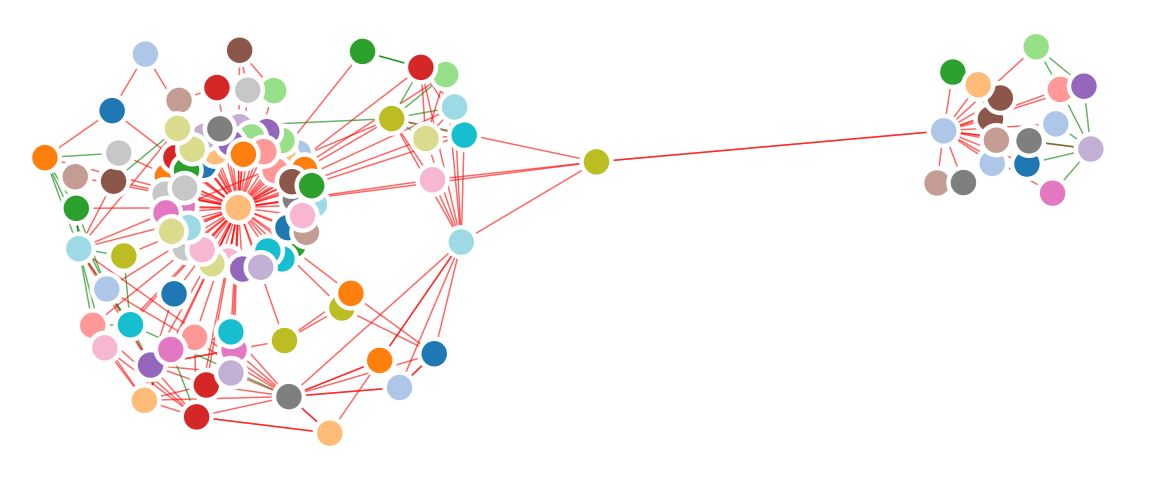
\includegraphics[scale=0.5]{img/graph.JPG}
\end{figure}

Quelques précision sur le graphe : 
\begin{itemize}
\item Le graphe est dynamique, et un pointage du curseur sur un  nœud affiche le nom du QRT représenté.
\item la distance entre deux noeuds matérialise la force de leur lien. Plus les noeuds sont proche, plus ils existent des assertions qui relient ces QRT.
\end{itemize}

Ce graphe permet une représentation visuelle de l'ensemble des liens qui existent entre les QRT. A l'aide de ce graphe il est possible de distinguer les QRT centraux, c'est à dire ceux qui auront tendance à être la base des autres, et de pouvoir bien définir un ordre cohérent de remplissage des QRT afin d'éviter les erreurs.




\chapter{De SAS à Python}

Le logiciel utilisé pour réaliser l'inventaire, est SAS. Cependant la licence du logiciel ne sera pas renouvelée et python a été choisi comme alternative. Ainsi un des grands prochains chantier du service sera la migration du code SAS existant vers python, et d'en faire le langage spécial inventaire.

Pour décrire un peu l'inventaire, il consiste à faire l'état du portefeuille client, et de calculer certaines variables techniques pour chaque assuré. C'est donc un ensemble de requête, de manipulations, de calcul sur des tables (ajout de colonnes, groupes, jointures). 

Le but de la mission est de tester la faisabilité du chantier. Il s’agissait de comprendre l’ensemble des traitements effectués pour réaliser les inventaires avec SAS, s'assurer qu'ils sont réalisables sous python et de savoir comment les implémenter. 

Pour réaliser du traitement de données, il y a pandas. Pandas est une bibliothèque python pour la manipulation de données, c'est Wes McKinney, un statisticien américain qui en est le principale auteur. Ainsi toutes les manipulations qu'offre SAS pour l'inventaire sont réalisables sous python.


\chapter{Participation au bénéfice}

Le code des assurances à l'article L 331-3 stipule :
"Les entreprises d'assurance sur la vie ou de capitalisation doivent faire participer les assurés aux bénéfices techniques et financiers qu'elles réalisent, dans les conditions fixées par arrêté du ministre de l'économie et des finances."

Ainsi GGVie est en tant que société d'assurance vie, calcul chaque année la participation au bénéfice règlementaire qu'elle devra verser à ses assurés.

\section{Calcul de la participation au bénéfice règlementaire (PBR)}

L'objectif de cette mission était de concevoir un programme python qui calculerait la participation au bénéfice règlementaire en utilisant pour seule entrée la balance.
La balance est un journal comptable dans lequel est repertorié l'ensemble des flux financiers liés à l'activité de la société d'assurance.

Le calcul de la participation au bénéfice règlementaire, se fait à parir d'un compte de participation au résultat qui se présente comme suit : 

\begin{table}[H]
\centering
\caption{Compte de participation aux résultats}
\label{CPR}
\begin{tabular}{|l|L{9cm}|L{4cm}|}
\hline
 & \multicolumn{1}{c|}{RUBRIQUE}  & \multicolumn{1}{c|}{COMMENTAIRES} \\ \hline
1 & Primes &  \\ \hline
2 & Charges des prestations &  \\ \hline
3 & Charge des provisions d'assurance Vie et des autres provisions techniques &  \\ \hline
A. & Solde de souscription (2) & 1-2-3 \\ \hline
5 & Frais d'acquisition &  \\ \hline
6 & Autres charges de gestion nettes & 5+6 \\ \hline
B & Charges d'acquisition et de gestion nettes &  \\ \hline
Gt & Participation de l'assureur aux bénéfices de la gestion techniques (A 331-4) & Gt = 10\% de (A-B) si A-B >0. Gt = 0 si A-B<0 \\ \hline
Pf & Part des produits financiers & Pf = 85\% du solde du compte financier \\ \hline
R & Solde de réassurance cédée &  \\ \hline
N & Solde débiteur du compte de participation aux résultats de l'exercice précédent &  \\ \hline
Sr & Solde du compte de participation aux résultats & A - B - Gt + Pf + R - N \\ \hline
lt & intérêts crédités aux provisions mathématiques &  \\ \hline
Mm & Montant minimal annuel de la partcipation aux bénéfices & Mm = Sr - It \\ \hline
\end{tabular}
\end{table}

Les rubriques du tableau \ref{CPR} \footnote{AXA, Befec-PriceWaterhouse, NORMES ET REGLEMENTATION CMPTABLES, L'Argus, 1996} peuvent être obtenues à partir du compte de résultat et leurs calculs sont définis par le code des assurances.

\section{Calcul de la PBR avec python}

Le calcul de la PBR se fait dans un classeur excel se servant de données d'autres classeurs maintenus par équipes différentes. Cependant cette méthode présente la conséquence d'un procédé long, impliquant plusieurs intermédiaires résultant sur un  risque aggravé d'erreur de calculs. C'est une vrai usine à gaz, difficile d'y voir claire au premier coup d'oeil.

L'objectif est donc d'écrire un programme python qui élimine l'ensemble de ces intermédiaires, qui se contente de la balance, pour calculer la PBR.

Pour commencer, j'ai élaborer le compte de résultat à partir de sa maquette. 
La maquette du compte de résultat est un tableau qui associe chaque poste du compte de résultat aux comptes qui la compose.

Ensuite à partir du compte de résultat il reste à construire le compte de participation aux résultats. 
Cependant, certaines rubriques du compte de participation aux résultats ne sont pas explicites dans le compte de résultat, il faut donc faire une correspondance entre les rubriques des deux comptes. Une tache pas très aisé du fait qu'il est difficile de trouver des personnes sources unanimes.

Une autre approche consiste à décortiquer les classeurs excel déjà en place qui calculent la PBR. c'est long et fastidieux, et en plus dans certains classeurs les céllules sont en "durs" plutôt que calculées. Conséquence, on se retrouve avec des quantités que l'on ne sais pas calculer. Et lorsque l'on se réfère au compte de participation au résultat pour calculer ces quantités, on se retrouve avec le problème de vocabulaire.

%\ref{CPR} que dans les classeurs excel déjà présents qui calculent la PBR.

Par exemple le solde de souscription dans le tableau \ref{CPR} est calculé différemment du solde de souscription dans les classeurs. En outre, le solde de souscription est appelé intérêt technique dans certains classeurs.

En résumé, il n'existe pas un vocablaire explicite, entre la maquette du compte de résultat, le code des assurances, et des différents classeurs déjà utilisés pour calculer.

De cette mission, j’apprends que dans le monde de l'entreprise on peut se retrouver avec des missions qui paraissent simples au départ, mais qui finissent par se révéler très complexe au point de déboucher dans des impasses.

\chapter{Le Challenge R de Groupama}

La direction internationale du Groupe GROUPAMA a lancé au début de l'année 2017 un concours de data science entre toutes les entités et filiales du groupe baptisé le "Challenge R". L'idée de ce concours était de permettre aux différentes entités de développer eux même une solution à un problème concret tout en utilisant des outils open source et des techniques modernes d'apprentissage automatique.

Le service de veille réglementaire et technologique a représenté GGVie au Challenge R. Ayant été soumis à des problèmes de données anormaux dans les tâches de gestion actif-passif, mon tuteur a donc eu l'idée d'un outils de détection d'anomalies dans des données en utilisant des méthodes d'apprentissage automatique. J'étais donc  chargé de l'implémentation en python et de la recherche de toutes méthode ou technique pouvant mener à un modèles robuste et fiable.

\section{Modélisation du passif avec MoSes}

La modélisation du passif consiste à projeter le portefeuille d'une ou plusieurs police d'assurance sur quarante (40) ans, dans le but d’observer des postes du passif, et d'anticiper les engagements et les rendements futurs.
Une sortie de modélisation du passif d'une police d'assurance, sera un ensemble de séries chronologiques, chacune représentant la projection d'un poste du passif de cette police. 
A titre d'exemple, considérons la police d'assurance AX1, la modélisation de son passif sur 40 ans aura la forme suivante : 
% Ce tableau est utilisé pour donner un aperçu du type de données obtenu en sortie de modèle
\begin{table}[H]
\centering
\caption{Passif de la police d'assurance \textsc{AX1}}
\label{my-label}
\begin{tabular}{|l|l|l|l|}
\hline
    &  2018   &  2019   &  20..  \\ \hline
 MARGE TECHNIQUE   &  .   &   .  &  ...  \\ \hline
 PROVISIONS TECHNIQUES  &  .   &  .   &  ...  \\ \hline
 CHARGE DE PARTICIPATION AUX BENEFICES  &   .  &   .  &  ...  \\ \hline
  ...  &  .   &  .   &   ... \\ \hline
\end{tabular}
\end{table}

La projection du passif se fait avec le logiciel de gestion actif-passif MoSes de chez Towers Watson. Afin de fournir des projections, MoSes prend comme données d'entré :

\begin{itemize}
\item le portefeuille dont on désire projeter le passif dans le temps
\item un ensemble d'hypothèses qui se présente sous la forme de tableaux de probabilité qu'un assuré change d'état d'une année à l'autre.
\end{itemize}

Pour chaque année de projection MoSes, applique les hypothèses au portefeuille pour simuler les changements d'états (décès, invalidité, incapacité...) des assurés d'une année à l'autre. Pour chaque année de projection, une simulation des flux de trésorerie engendré par les variations du  portefeuille, permet de construire le passif correspondant. 

\section{Problématique}

La modélisation de l'ensemble des polices pour un même poste du passif présente souvent des sorties "étonnantes", on peut observer des particularités chez certaines séries pour un même poste de passif comme : 

\begin{itemize}
\item des séries chronologiques avec des sauts
\item des valeurs nulles en plein milieu de série
\item des séries aux tendances différentes 
\item ...
\end{itemize}

Ces erreurs dans les résultats de modélisation peuvent engendrer des écart de prévision et de gestion de risques, d'où l'idée de construire un modèle de détection d'anomalie qui sera présenté au concours de data science.

Ce modèle, baptisé "Garbage in, Garbage out" (G.I.GO), s'inscrit dans un objectif de fiabilisation des données. Pour prendre des décisions optimales basées sur des résultats fiables, il est essentiel que ces résultats proviennent du traitement de données fiables.

\section{Garbage in, Garbage out (Gigo)}

Gigo est un modèle qui détecte les anomalies dans les résultats de modélisation du passif en se basant sur la forme générale de toute les séries chronologiques.

La construction du modèle s'est effectué essentiellement sous deux approches partant de différentes hypothèses et interprétation afin de construire un modèle fiable et performant. 

\subsection{Aproche basé sur la forme générale des courbes chronologiques}

La première approche a consisté à supposer que la détection pourrait se faire à partir de la forme générale des courbes des séries chronologiques. 

Supposons un ensemble de simulation d'un poste du passif pour 50 produits d'assurance différents. On aura donc 50 séries chronologiques, chacune représentant la projection dans le temps de différents produits pour un même poste du passif.

Chaque série présentera donc une forme générale, elle seront soit croissantes, décroissantes, convexes, concaves, ou une combinaison de ces formes.

\subsubsection{Détection des formes : le modéle de Nielson-Siegel-Svensson}

Partant de l'objectif d'une détection de séries anormales basées sur leur forme, la première étape consistera donc à modéliser la forme générale des courbes. Pour ce faire, on utilisera le modéle de Nielson Siegle Svensson (NSS).

Le modèle de Nielson Siegel Svensson (NSS) est une extensions du modéle de Nelson and Siegel (1987) par Svensson (1994), il est utilisé par la Banque Centrale Européenne (BCE) pour construire la courbe des taux. 

Le modéle propose une modélisation de la courbe des taux en fonction des maturités par l'équation\footnote{Manfred Gilli, Stefan Große and Enrico Schumann, "Calibrating the Nelson–Siegel–Svensson model", 30/03/2010} :

\begin{multline}
y(\tau)=\beta_{0}+\beta_{1}\left[\frac{1-exp(\frac{-\tau}{\alpha_{1}})}{\frac{\tau}{\alpha_{1}}}\right]+\beta_{2}\left[\frac{1-exp(\frac{-\tau}{\alpha_{1}})}{\frac{\tau}{\alpha_{1}}}-exp(\frac{-\tau}{\alpha_{1}})\right]+ \\
\beta_{4}\left[\frac{1-exp(\frac{-\tau}{\alpha_{2}})}{\frac{\tau}{\alpha_{2}}}-exp(\frac{-\tau}{\alpha_{2}})\right]
\label{nss}
\end{multline}

Ainsi la calibration du modèle se fait par l'estimation des paramètres : $ \beta_{0},\beta_{1},\beta_{2},\beta_{3},\alpha_{1},\alpha_{2}. $ (Avec $ \tau $ la maturité)

Le modéle est à la base destiné à resoudre un problème de finance. Cependant, il présente un aspect qui nous permet de l'adapter à notre contexte de détection d'anomalies. En effet les paramétres $ \beta_{0},\beta_{1},\beta_{2},\beta_{3},\alpha_{1},\alpha_{2}. $  représentent chacun un aspect de la forme de la courbe modélisée. Ainsi, nous pouvons supposer que ces six paramètres résument bien la forme générale de la courbe qu'elle modélise. 

Pour revenir à notre contexte, nous pouvons donc résumer une série chronologique d'une quarantaine de points à six paramètres essentiels qui traduise sa forme.

\subsubsection{Adaptation au modèle NSS}

Le modèle NSS a été construit afin de modéliser des taux en fonction de leur maturité. Dans notre contexte nous avons des quantité de passifs à l'ordre de plusieurs millions pour chaque année futur. Ainsi pour se conformer au modéle, il est nécessaire de ramener ces quantités à une echelle de taux (entre -1 et 1), et de ramener les années à des maturités.

\subsubsection{Calibration du modèle NSS}

Afin de trouver les six paramètres il faut procéder par la calibration du modèle. La calibration du modèle se fait par optimisation, il faut trouver les paramètres qui font passer la courbe de la fonction \eqref{nss} au mieux par l'ensemble des points de la série chronologique. 

Pour estimer les six paramètres on résout le problème d'optimisation qui consiste à minimiser les distances entre la fonction de NSS et les points à interpoler. La fonction objective sera donc :

\begin{equation}
min\sum_{k=1}^n (y_{nss}-y_{obervation})^{2}
\label{obj}
\end{equation}

sous les contraintes : $ \beta_{1} > 0; \lambda_{1,2} > 0; \beta_{1}+\beta_{2}>0 $

Le problème d'optimisation n'est pas convexe, une méthode "classique" de résolution se limiterait à trouver des optimum locaux. C'est pourquoi une méta-heuristique\footnote{"Une métaheuristique est un algorithme d’optimisation visant à résoudre des problèmes d’optimisation difficile" : https://fr.wikipedia.org/wiki/Métaheuristique}, en l’occurrence l'évolution différentielle\footnote{Rainer STORN and Kenneth PRICE : "Differential Evolution – A Simple and Efficient Heuristic for Global Optimization over Continuous Spaces", 1997} sera utilisée afin de trouver un optimum global.

En appliquant la méthode d'évolution différentielle afin de minimiser la fonction objective, on obtient comme solution le vecteur des six paramètres.

Appliquer le modèle NSS aux séries chronologiques revient à les réduire à six principaux paramètres qui résument au mieux leur forme.
\subsubsection{Application de NSS}

Soit la série chrnologique suivante...

\begin{figure}[H]
\centering
\caption{Série chronologique normalisée}
   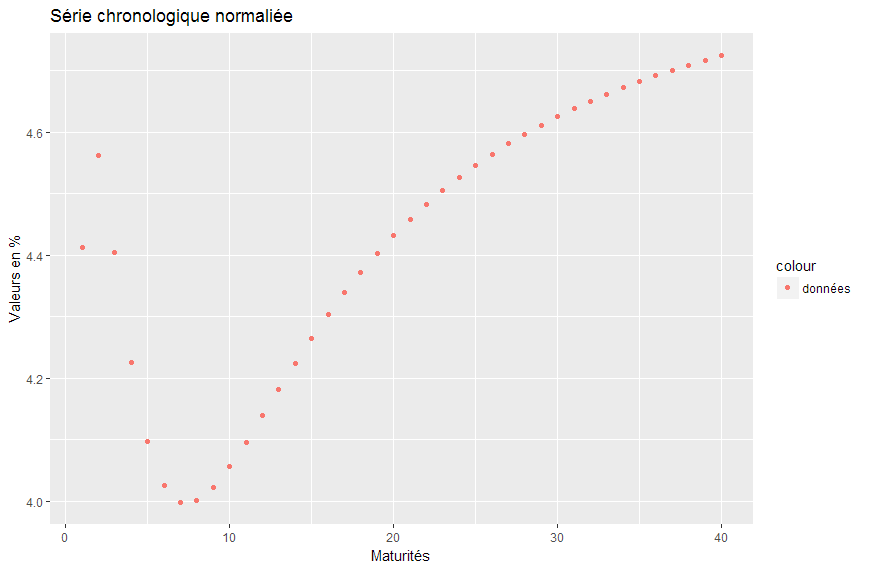
\includegraphics[scale=0.7]{img/data.png}
\end{figure}

En calibrant NSS sur ces données, on peut en déduire sa forme principale, à partir des six paramètres du modèle de nielson Siegel Svensson que l'on obtiendra.

Après calibration on obtient les six paramètres de l'équation de NSS, à partir de ces six paramètres et des maturités on recalcule les valeurs de la séries normalisée afin d'évaluer de façon graphique les performances de la calibration. En supperposant les série normalisée initiale et la série obtenue par estimation de NSS, on obtient le graphique suivant :

\begin{figure}[H]
\centering
\caption{Série chronologique normalisée reprise par le modèle NSS}
   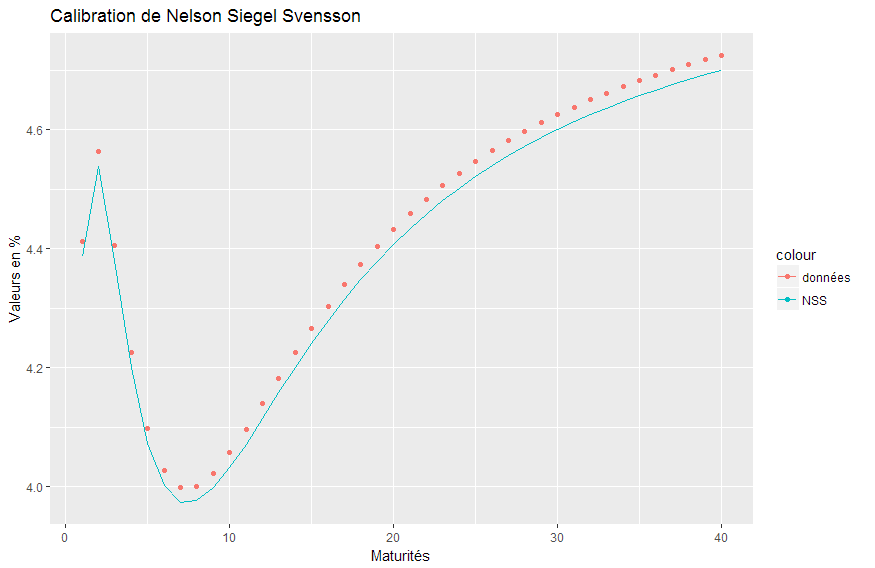
\includegraphics[scale=0.7]{img/nss.png}
\end{figure}

Les six paramètres optimaux de l'équation de NSS, obtenues à partir de la calibration du modèle sont : 

\begin{table}[H]
\centering
\caption{Paramètres optimaux}
\label{my-label}
\begin{tabular}{|l|r|l|l|l|l|l|}
\hline
$\beta$ & $\beta_0$ & $\beta_1 $ & $\beta_2$ & $\beta_3$ & $\alpha_1$ & $\alpha_2$ \\ \hline
Valeurs & 5 & -2 & 5 & -5 & 1 & 3 \\ \hline
\end{tabular}
\end{table}

Sans passer par tous les points, observe que le modèle trace une courbe épouse bien la l'allure de la forme de la série chonologique normalisée, comme une ombre. Ainsi on déduit que le modèle de NSS viens de réduire à six paramètres la forme d'une courbe de quarante points.

Maintenant évaluons notre déduction en testant l'effet de changement de chacun des paramètres sur la courbe obtenue tracée par les paramètres. L'idée est de confirmé, q'un changement de paramètre abouti à une nouvelle courbe d'un forme plus ou moins différente.

En effectuant successivement un changement de l'un des six paramètres afin d'évaluer le changement de courbe obtenu, on obtient les graphiques suivants :

\begin{figure}[H]
\centering
\caption{Conséquences des changements de paramètres}
   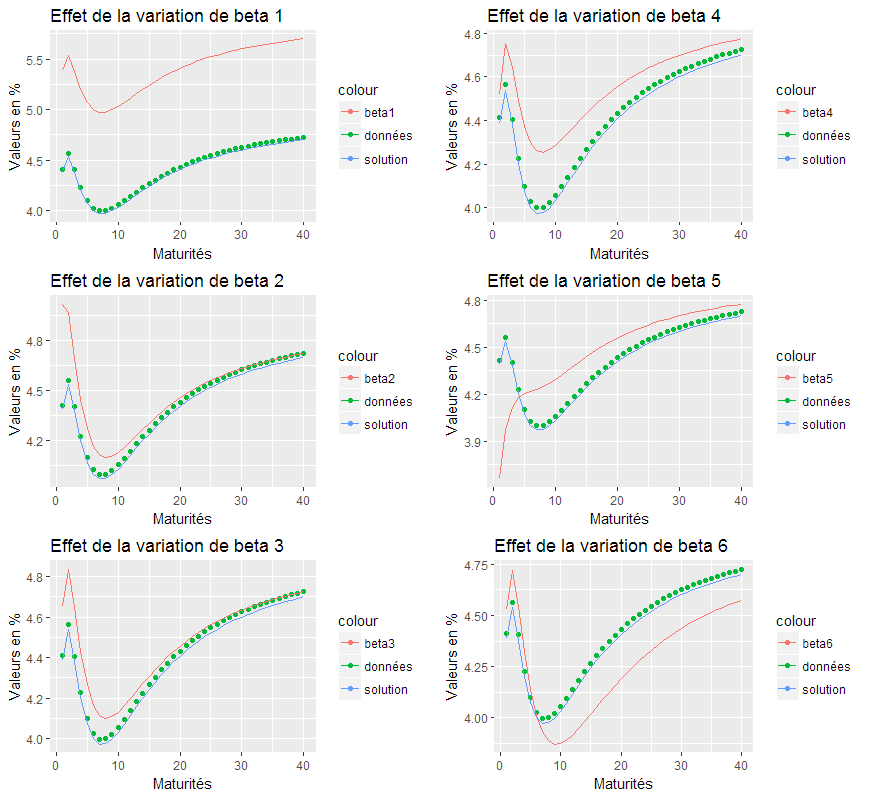
\includegraphics[scale=0.7]{img/betas.png}
\end{figure}

La modification qui a été faite est que l'on a successivement ajouté à chaque paramètre la valeur de 1.
Pour chaque paramètre modifié, on observe bien certains changements dans la forme de la courbe, ce qui signifie bien que les six paramètres permettent de caractériser une courbe particulière.

En résumant une courbe à ses six paramètres, on effectue une réduction de dimension, mais aussi un changement de repère, on passe des valeurs de la courbe, à la forme de la courbe. Ainsi, calculer la distance entre les paramètres de deux courbes différentes reviendrait à calculer la différence qui existe entre les formes de leurs courbes respectives.

\subsubsection{Détection}

Après avoir identifié la forme de la courbe de chaque série, on passe maintenant à la phase de détection d'anomalies. La détection d'anomalie est un procédé utilisé dans des domaines divers, dans le but essentiel d'isoler des comportements ou des individus "suspects" dans un ensemble de données ou d'activités. Dans un ensemble de données, les anomalies seront très peu, et différentes ou inhabituelles. 

Il existe une multitude de méthode de détection d'anomalies, toutes en générale basée sur les calculs de distances et de noyaux. La méthode que nous allons utiliser procède à la détection d'anomalie en utilisant une approche aléatoire, appelé forêt d'isolation. La seconda partie du rapport sera consacrée au développement théorique de cette méthode.

\subsection{Approche basée sur les séries chronologiques}

Par cette approche on procède directement à l'application de la méthode de forêt d'isolation pour détecter les anomalies, sans étape intermédiaire en supposant que les années de projection sont des variables. Cette approche sera dévéloppée dans la seconde partie.

L'objectif de la seconde partie sera de présenter l'aspect théorique et pratique, montrant les performances et l'intérêt de cette méthode dite de machine learning dans un contexte de la finance de marché par exemple.


%In this section, we will deal with the optimisation problem, so our aim will be to solve
%model (3). The problem is not convex, so we will use appropriate procedures: optimisation
%heuristics (Gilli and Winker, 2009). More specifically, we will apply Differential Evolution
%(de; Storn and Price, 1997). We will not discuss the algorithm in detail here; the implementation
%follows the pseudocode given in Gilli and Schumann (2010 (in press). R-code is given
%in the appendix and can be downloaded from http://comisef.eu .
% part  (end)/

\part{Détection d'anomalies}
\label{prt:detection}

\chapter{La détection d'anomalies par Isolation} 

\section{Méthode d'isolation des anomalies}

Dans un ensemble de données, les anomalies peu nombreuses avec des caractéristiques très différentes.

La détection d'anomalies, consiste à isoler ces données rares et fortement différentes d'une base de données. C'est un concept utilisé dans différents domaines comme la sécurité informatique (détection d'intrusion, ),.

Il existe une multitude de méthodes de détection d'anomalies, toutes basées en générale sur les calculs de distance ou de noyaux. Ces méthodes supposent que des données "normales" auront tendance à être fortement groupées, rapprochées et les données qui sont éloignées d'un ou de plusieurs groupes de données sont considérées comme des anomalies.

Sachant que dans un ensemble de données, les anomalies sont plus ou moins très rares et différentes, la méthode procède par isolation pour détecter ses anomalies. L'isolation consiste à construire un arbre de décision à partir des données jusqu'à ce que chaque individu soit dans une et une seule feuille.

Une fois que les données sont isolées dans l'arbre de décision ou d'isolation, la probabilité qu'une donnée soit une anomalie est quantifiée par sa profondeur dans l'arbre. Une données qui a été isolée très vite lors de la construction de l'arbre de décision a plus de probabilité d'être une anomalie.

Pour effectuer la détection d'anomalies par isolation, on choisi au hasard un échantillon dans une base de données, ensuite on choisi des variables au hasard parmi les variables de l'échantillon et on déroule un arbre de décision.

%On répète cette méthode n fois, on crée donc $n$ arbres d'isolation %et d'échantillons différents tous tirés des données initiales. %L'ensemble de ces arbres d'isolations est appelé forêt d'isolation.

\section{Phase d'apprentissage}

La phase d'apprentissage consiste à construire un ensemble d'arbre soit des \emph{iTree}, sur les données pour créer une forêt d'isolation, les \emph{iForest}.

Le principe est relativement simple, et s'effectue essentiellement en deux phases dont la première sera la construction de l'arbre de décision, puis par bootstrapping la construction de la forêt de décision.

\subsection*{Construction de l'arbre de décision}

La construction de l'arbre d'isolation se fait par échantillonnage sur les deux dimensions, variables et individus.
Considérons la base de données  suivante :
Elle est formée de $m$ individus $I$ et de $n$ variables $V$.

\begin{table}[H]
\centering
\caption{Base de données}
\label{bdd}
\begin{tabular}{|l|l|l|l|l|}
\hline
 & $V_1$ & $V_2$ & $\cdots$ & $V_n$ \\ \hline
$I_1$ &  &  &  &  \\ \hline
$I_2$ &  &  &  &  \\ \hline
$\vdots$ &  &  &  &  \\ \hline
$I_m$ &  &  &  &  \\ \hline
\end{tabular}
\end{table}

Premièrement, un échantillonnage est effectué de façon aléatoire, sur les individus et sur les variables qui les caractérisent.

\begin{table}[H]
\centering
\caption{Échantillon}
\label{ech}
\begin{tabular}{|l|l|l|l|}
\hline
 & $V_1$ &  $\cdots$ & $V_n$ \\ \hline
$I_1$ &  &  &  \\ \hline
$\vdots$ &  &  &  \\ \hline
$I_m$ &  &  &  \\ \hline
\end{tabular}
\end{table}

A partir de l'échantillon choisi de façon aléatoire, un arbre d'isolation (décision) est construit, de telle sorte que chaque individu se trouve seul sur une feuille au bout de l'arbre. c'est la condition d'arrêt de la construction d'un arbre, mais toute fois elle peut être manipulée de telle sorte à pouvoir arrêter la construction d'un arbre trop profond.

Dans la phase d'apprentissage, trois paramètres sont donc nécessaires pour le déroulement de l'algorithme : 

\begin{itemize}
    \item $X$ : les données
    \item $\psi$ : la taille de l'échantillon
\end{itemize}

La taille de l'échantillon $\psi$ permet de contrôler la taille des données d'apprentissage. C'est un paramètre qui joue donc notamment sur la profondeur de l'arbre d'isolation et donc sur la performance de la méthode d'isolation. Par ailleurs, à partir d'une certaine taille, les performances de détections tendent à devenir constante, généralement $\psi=256$ est suffisant pour effectuer une détection d'anomalie dans une base de données.

\subsection*{Construction de la forêt d'arbre de décision}
Une forêt d'arbre de décision est composée de plusieurs arbres de décision. Sa construction s'effectue en ré-échantillonnant plusieurs fois avec la construction d'un arbre par échantillon. Ainsi, un autre paramètre vient s'ajouter aux deux autres, $t$ qui désigne le nombre d'arbre qui compose la forêt. En générale, le chemin d'isolation d'un individu dans un arbre converge avant la construction de $t=100$ arbres.
\\
\\
La complexité dans le pire des cas ce la phase d'apprentissage est de $O(t\psi^2)$ et temps, et de $O(t\psi)$ en espace.

\section{Phase d'évaluation}
La phase d'évaluation consiste à calculer le taille moyenne du chemin d'isolation d'un individu sur l'ensemble de la forêt.
La taille $h(x)$ du chemin d'un individu $I$, correspond au nombre de noeuds $e$, entre la base de l'arbre d'isolation et le noeud d'extrémité (bout de l'arbre) où cet individu a été isolé. 
Lorsque la taille du chemin d'isolation d'un individu dépasse une certaine limite $hlim$ prédéterminée, la taille du chemin est estimée par $hlim+c(Size)$, avec $c(Size)$ une valeur d'ajustement \footnote{\cite{Liu2012}}.
\\
\\
La complexité dans le pire des cas ce la phase d'évaluation est de $O(nt\psi)$ et temps, avec $n$ le nombre de test.

\section{Les anomalies et leurs scores}

Un score, pour déterminer le degré d'anormalité d'un individu est essentiel à toute méthode de détection d'anomalie.
Le score $s$ d'un individu I se calcul comme :
\begin{equation}
    s(I,\psi)=2^\frac{E(h(x))}{c(\psi=)}
\end{equation}

\begin{itemize}
    \item $E(h(x))$ est la moyenne des tailles du chemin d'isolation d'un individu I dans une forêt d'isolation.
    \item $c(\psi)$ désigne la moyenne des $h(x)$ dans un échantillon
\end{itemize}

Dans certaines conditions la valeur du score est directement déduite :
\begin{itemize}
    \item $E(h(x)) \rightarrow 0,  s \rightarrow 1;$
    \item $E(h(x)) \rightarrow \psi-1,  s \rightarrow 0; $
    \item $E(h(x)) \rightarrow c(\psi),  s \rightarrow 0.5;$
\end{itemize}

\chapter{Application}

Ce chapitre se consacre à une application pratique de la détection d'anomalies dans un contexte de finance de marché et de gestion du risque. 

Maintenant que nous disposons d'un algorithme peu coûteux en temps et en mémoire, on peut poser des hypothèses de détection d'anomalies que nous allons appliquer à des données financières de marchée volumineuse, pour en détecter ce qui s'éloignent de la norme. Dans un certain contexte on ne parlera pas d'anomalies bien que nous appliquons une méthode de détection d'anomalie, mais plutôt de particularité.

\section{Le Standard \& Poor's 500}

Le Standard \& Poor's 500 ou S\&P 500 est un indice bousier basé sur un peu plus de 500 grandes sociétés cotées sur les bourses des États-Unis.
\\
\\
Considérons l'historique des prix de clôture du marché de l'ensemble des actifs de l'indice entre le 11 Août 2015 et le  11 Août 2017. L'objectif de cette application, sera de détecter parmi les 500 actifs, les quelques uns qui ont des comportements très particuliers sur le marché.
\\
\\
Cependant, il est nécessaire de noter que les interprétations sur les actifs anormaux dépendent fortement des variable qui caractérisent les actifs. Une donnée peut être identifiée pour être anormale, mais l'essentiel sera de savoir dans quelle contexte elle est anormale.
\\
\\
En fonction du type d'anomalie que l'on veut identifier, il faut veiller à travailler sur les bonnes variables, au risque de considérer des anomalies et résoudre les mauvais problèmes.
\\
\\
Notre objectif sera de détecter des actifs qui présentent des distributions de rendement anormaux sachant que par hypothèse les rendements historiques d'un actif suivent une loi normale centrée en zéro, c'est à dire que son espérance est nulle, avec une volatilité proportionnelle au temps. L'objectif de cette application est de savoir si il existe des actifs de l'indice S\&P 500 qui présentent une loi normale de caractéristique extrême par rapport aux autres, synonyme de plus ou moins de risque.

\section{Isolation sur le Standard \& Poor's 500}

Soit les 500 actifs qui composent l'indice S\&P 500. 
Considérons l'historique des prix de clôture des actifs entre le 11 Août 2015 et le  11 Août 2017.
Cette application porte sur une étude des distributions des rendements de ces actifs, sachant que le rendement d'un actif suit une loi normale. 

\subsection{Les rendements}

Le graphique suivant montre l'évolution des rendements moyens entre le 11 Août 2015 et le 11 Août 2017. Le rendement moyen est le rendement journalier sur lequel on applique une moyenne mobile avec une fenêtre de quarante jours.

\begin{figure}[H]
\centering
\caption{Moyenne mobile des rendements}
   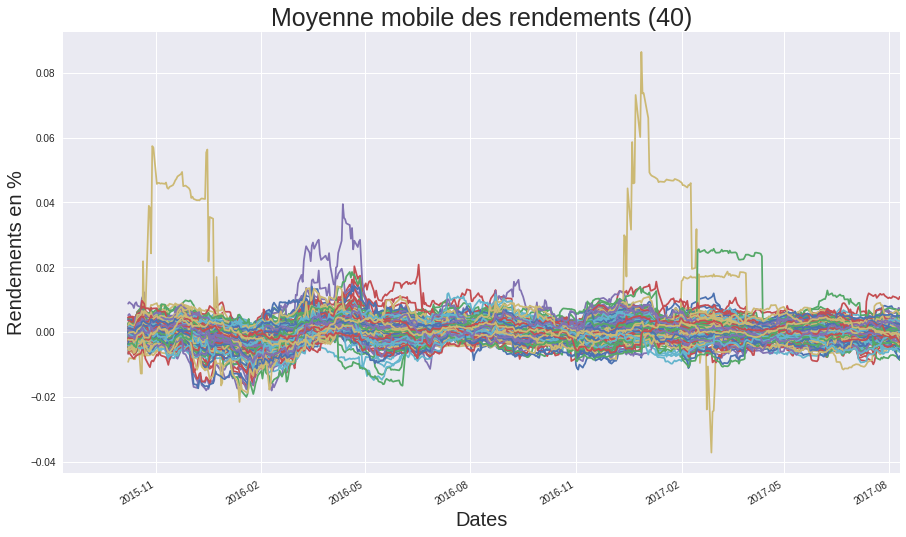
\includegraphics[scale=0.5]{img/rendements.png}
\end{figure}

Ce graphique est touffu et pratiquement illisible, on a superposé 500 courbes et on en distingue clairement aucune. Cependant, en regardant hors des surcharges, on peu remarquer quelques courbes qui se distinguent fortement avec des piques bien au dessus et ou au dessous de la moyenne des autres. Ce sont ces genres d'actifs que l'on veut détecter, les actifs avec un profil historique de rendement moyen totalement différent voir exceptionnel des autres. Une fois détecté, un ensemble d'étude peuvent être menées pour interpréter ces résultats.

\subsection{Les volatilités}

Le graphique suivant montre l'évolution des volatilités des rendements moyens entre le 11 Août 2015 et le 11 Août 2017. La volatilité moyenne mobile sur une fenêtre de quarante jour.

\begin{figure}[H]
\centering
\caption{Volatilité des actifs}
   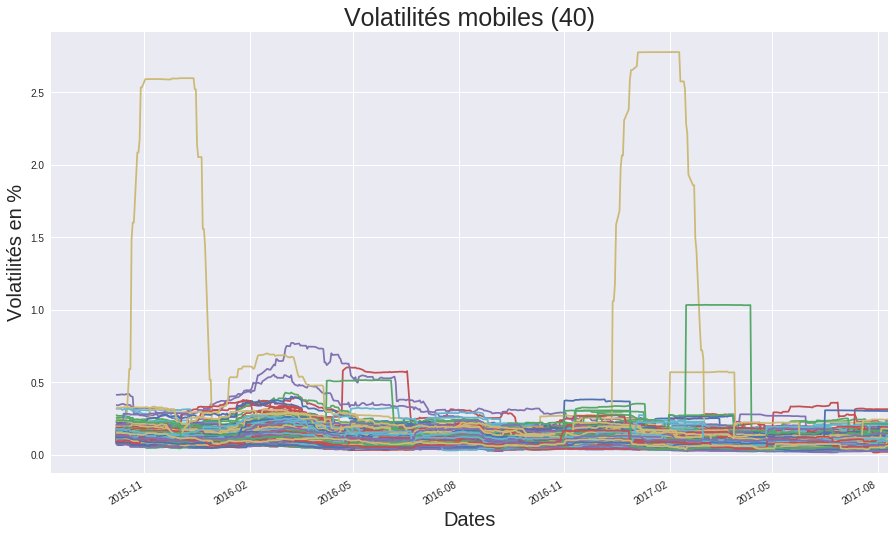
\includegraphics[scale=0.5]{img/volatilites.png}
\end{figure}

On observe une masse bien dense de courbe qui se superposent puis quelques unes qui se démarquent clairement par endroit.
Sachant que la volatilité d'un actif détermine le niveau de risque de ce actif, il n'est pas exagéré de vouloir porter un œil sur ce actif afin d'en évaluer efficacement le risque.

\subsection{Densité de probabilité des rendements}

Les rendements d'un actif suivent une loi normale centrée en 0 avec une certaine volatilité.  Les paramètres donc de volatilité et de rendements caractérisent la densité de la loi que suivra les rendements. C'est à dire qu'en étudiant la fonction de densité des rendements des actifs on porte aussi un œil sur ses deux premiers paramètres

La fonction de densité d'un actif dans cette application à été approximé de manière non paramétrique par la méthode d'estimation par noyaux\footnote{ Méthode de Parzen-Rosenblatt (wikipedia)}. Cette méthode est implémentée dans trois bibliothèque python et sont accessible de façon simple.

En utilisant cette méthode pour obtenir la courbe des distributions et en les superposant il est difficile de voir les différences entre les différentes distributions, elles ont l'air homogènes et de loi normale.

\begin{figure}[H]
\centering
\caption{Distribution des rendements}
   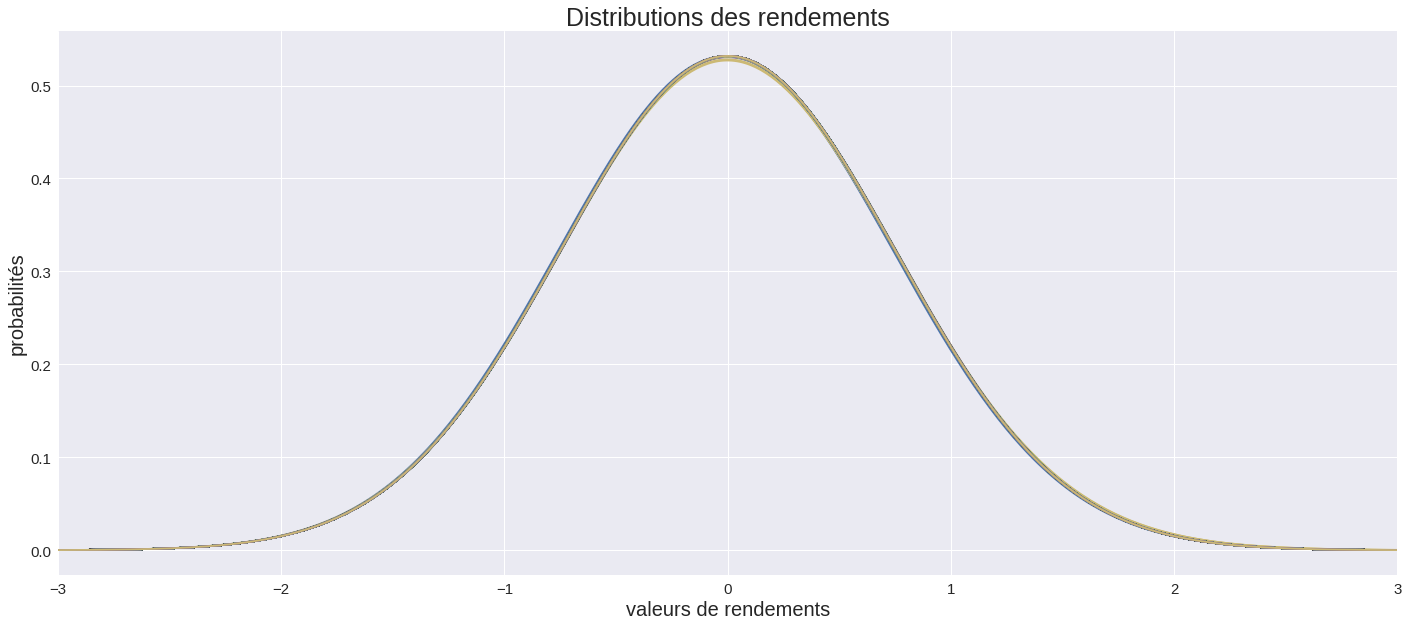
\includegraphics[scale=0.35]{img/distrib.png}
\end{figure}

\subsection{Densité par la méthode des histogrammes}

En regardant de plus près, en visualisant de façon empirique les différentes distributions, en utilisant un graphique d’histogramme lissé on aperçoit qu'en réalité les loi de probabilités des rendements sont différentes. Les différences se situent notamment soit à la base, au sommet et à la forme. Certaines distributions sont plus effilées que d'autres. 

La figure ce dessous illustre les différences de distribution de rendements entre 4 quatre  actifs qui composent le S\&P 500 choisies aléatoirement.

Ces actifs sont listés dans le tableau \ref{actif}.

\begin{table}[H]
\centering
\caption{Actifs du S\&P 500}
\label{actif}
\begin{tabular}{|l|}
\hline
A : Agilent Technologies Inc \\
AKAM : Akamai Technologies Inc \\
ADSK : Autodesk Inc \\
AAP : Advance Auto Parts \\ \hline
\end{tabular}
\end{table}

\begin{figure}[H]
\centering
\caption{Distribution des rendements}
   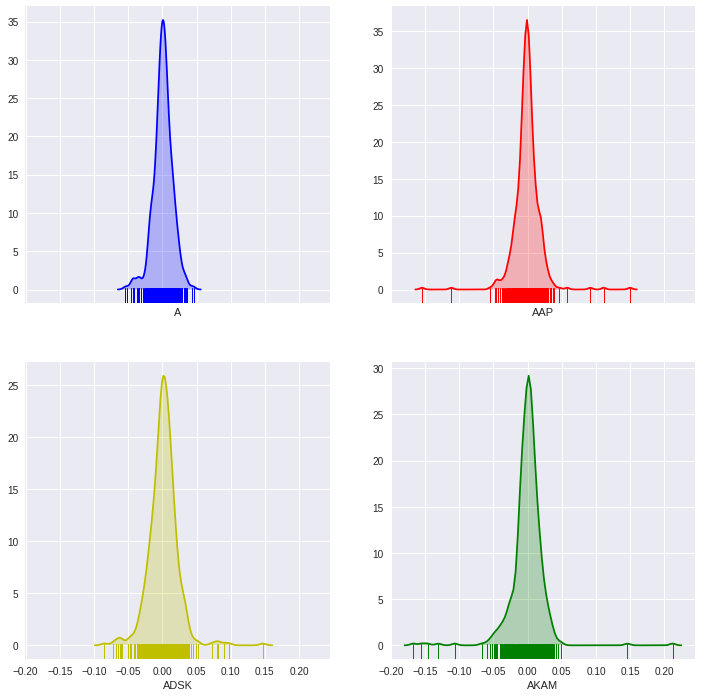
\includegraphics[scale=0.7]{img/distrib2.png}
\end{figure}

On peut noter que la loi des rendements n'est pas exactement normale, c'est une hypothèse, avec pour principale conséquence un biais dans la quantification de risque, notamment dans le calcul d'indicateur la Value at Risk (VaR).

Ces différentes courbes, apporte une précision sur la loi de probabilité des rendements de chaque actif avec les différences qui peuvent exister entre elles. Des différences qui peuvent principalement être interprétées comme une comparaison du niveau de risque. Certains actifs seront plus risqués que d'autres, et ceux qui présentent soit des niveaux de risque extrêmes (faibles ou élevé) peuvent être intéressant à détecter. C'est ainsi qu'intervient la détection d'anomalie, par une méthode qui va isoler ces actifs "particuliers", c'est à dire ceux avec un profil de rendement différent.

\section{Isolation des actifs}

La méthode de détection d'anomalie par isolation est implémentée  dans une librairie de machine learning python qui est Scikitlearn sous le nom de \emph{sklearn.ensemble.IsolationForest} \footnote{Documentation : http://scikit-learn.org/stable/modules/generated/sklearn.ensemble.IsolationForest.html\#id1}. 

Deux approches seront utilisées pour isoler les actifs qui présentent des "anomalies" de rendement. Une approche standard, directement appliquée sur la distribution des rendements puis une autre approche basée sur la forme de courbe de la distribution des rendements.

\subsection{Isolation des distributions}

En appliquant la méthode de détection d'anomalies par isolation,on obtient les actifs qu'elle aura isolé et qui donc présentent des différences signifiantes. Pour isoler ces actifs elle se base sur le score de chaque actif, ceux avec les scores les plus faibles ont une forte probabilité d'être des anomalies.

Ainsi l'ensemble des scores pour l'ensemble des actifs sont : 


\begin{figure}[H]
\centering
\caption{Scores de l'ensemble des actifs}
   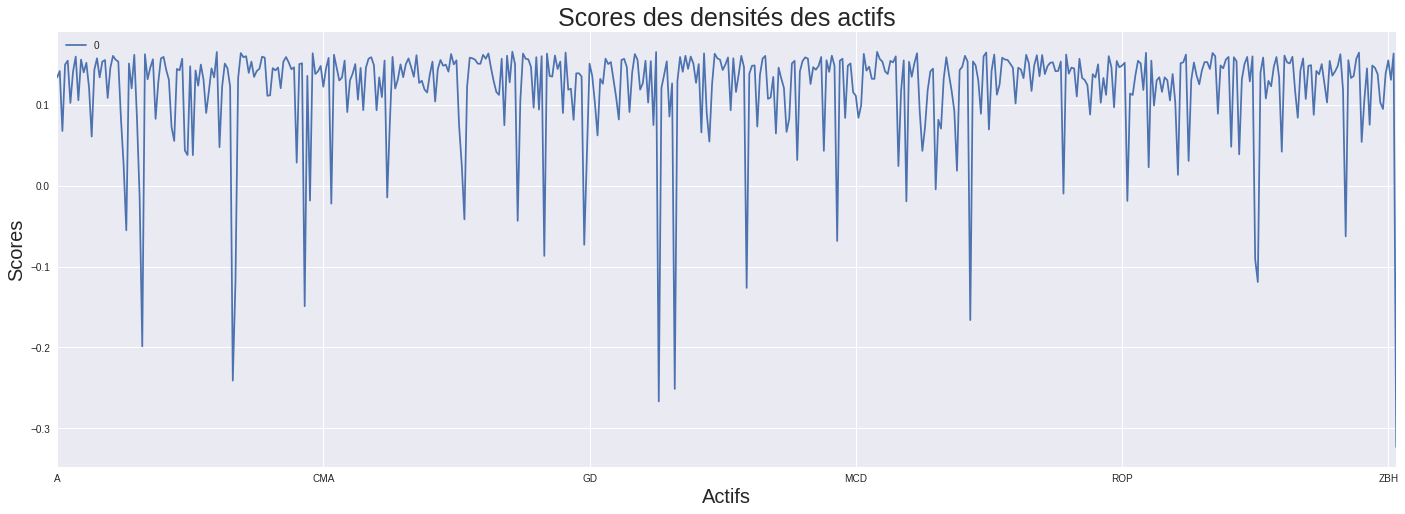
\includegraphics[scale=0.35]{img/scores_densite_all.png}
\end{figure}

Les scores des anomalies probables identifiées par la méthode se présente graphiquement comme ceci : 

\begin{figure}[H]
\centering
\caption{Scores des anomalies isolées}
   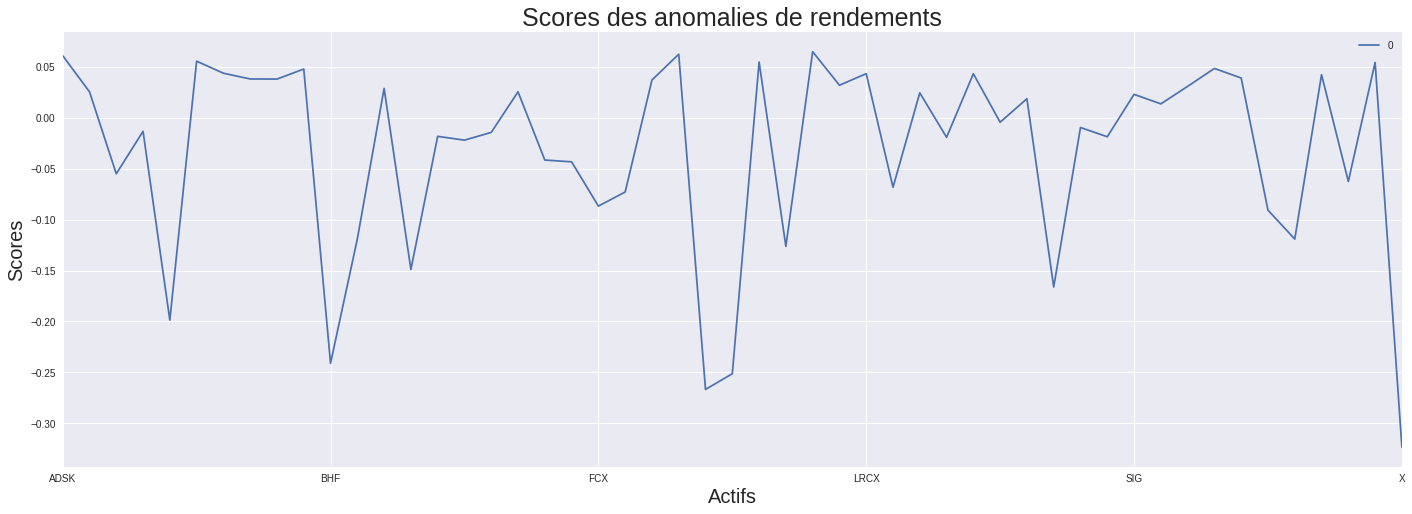
\includegraphics[scale=0.35]{img/scores_densite.png}
 \label{scoredensite}
\end{figure}

En conclusion la liste des anomalies identifiées avec leurs scores dans la figure \ref{scoredensite} est la suivante : 

['ADSK', 'ALB', 'ALGN', 'AMAT', 'AMD', 'APC', 'ARNC', 'ATVI', 'AVGO',
       'BBY', 'BHF', 'BHGE', 'CF', 'CHK', 'CHTR', 'CMG', 'CTXS', 'DVN', 'DXC',
       'EVHC', 'FCX', 'FTI', 'FTV', 'GILD', 'HLT', 'HPQ', 'INCY', 'JEC', 'KMI',
       'LB', 'LRCX', 'M', 'MOS', 'MRO', 'MU', 'NEM', 'NRG', 'NVDA', 'PRGO',
       'RRC', 'SIG', 'SRCL', 'STX', 'TRIP', 'TSCO', 'UA', 'UAA', 'URI', 'WMB',
       'WYNN', 'X']\footnote{ Les significations de ces abbréviations peuvent être trouvés sur http://www.zonebourse.com/S-P-500-4985/composition/}

\subsection{Identification des différences}

On retient donc que ces actifs listés ci dessus présenteront des distributions peu communes de l'ensemble des 500 actifs du S\&P 500 considérés au départ.
Maintenant clarifions un peu le tout par une comparaison entre distribution "normale" et "anormale".

Soit les actifs anormaux qui ont été isolés 'ALGN' et 'ADSK'. 
\\
Soit les actifs normaux 'A' et 'ABBV'.

Une comparaison des distributions de ces quatre actifs donne le graphique suivant : 

\begin{figure}[H]
\centering
\caption{Comparaison entre actifs "anormales" et "normals"}
   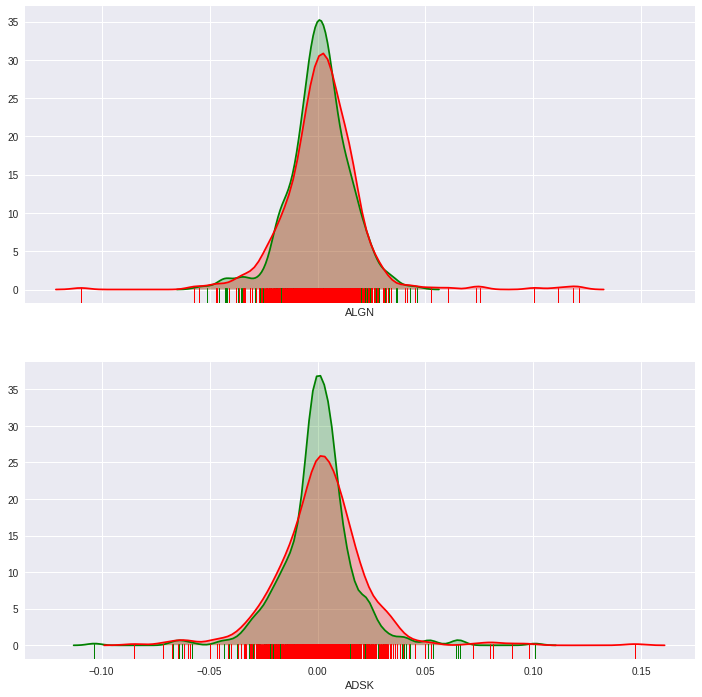
\includegraphics[scale=0.7]{img/anomalie_vs_normal.png}
 \label{anorm}
\end{figure}

Les courbes en vert présentent les distributions normales, et ceux en rouge les distributions isolées. La différence peut être résumé  comme suit :
\begin{itemize}
\item Les distributions normales (en vert dans la figure \ref{anorm}) ont des courbes avec une base fine, mais élancées en zéro
\item  Les distributions anormales (en rouge dans la figure \ref{anorm}) ont des courbes plus tassées en zéro avec une base plus épaisse.
\end{itemize}

A partir de ces différences identifiées, entre distribution de rendement normales et anormales on peu porter un ensemble d'interprétation sur ces allures et en identifier les conséquences.
La détection d'anomalie a été significative, elle a permit d'indexer directement des distributions de rendement particulières dans un ensemble, sans avoir à les comparer deux à deux.

\section{Isolation des actifs avec Nielson-Siegel-Svensson}

L'isolation par Nielson siegel svensson Consiste à recommencer le procédé de la section précédente savec différentes donnée. En effet, les distribution de probabilités sont passées à NSS, qui retourne les 6 coefficients pour chaque distribution qui résument la forme de sa courbe\footnote{L'application de la méthode de NSS sur l'historique des rendements pour les 500 actifs a duré 2 heures, pour un processeurs i7 quand core 2.6GHz }. On passe d'un historique de rendement sur deux ans, à essentiellement 6 variables sur lesquelles on applique la méthode de détection par isolation.

Il est important de préciser que les lois des rendements ont été estimées de façon non paramétrique en utilisant la méthode du noyau (méthode de Parzen-Rosenblatt).

On obtient les résultats suivants :

Score de l'ensemble des courbes de distribution.

\begin{figure}[H]
\centering
\caption{Scores de l'ensemble des distribution (NSS)}
   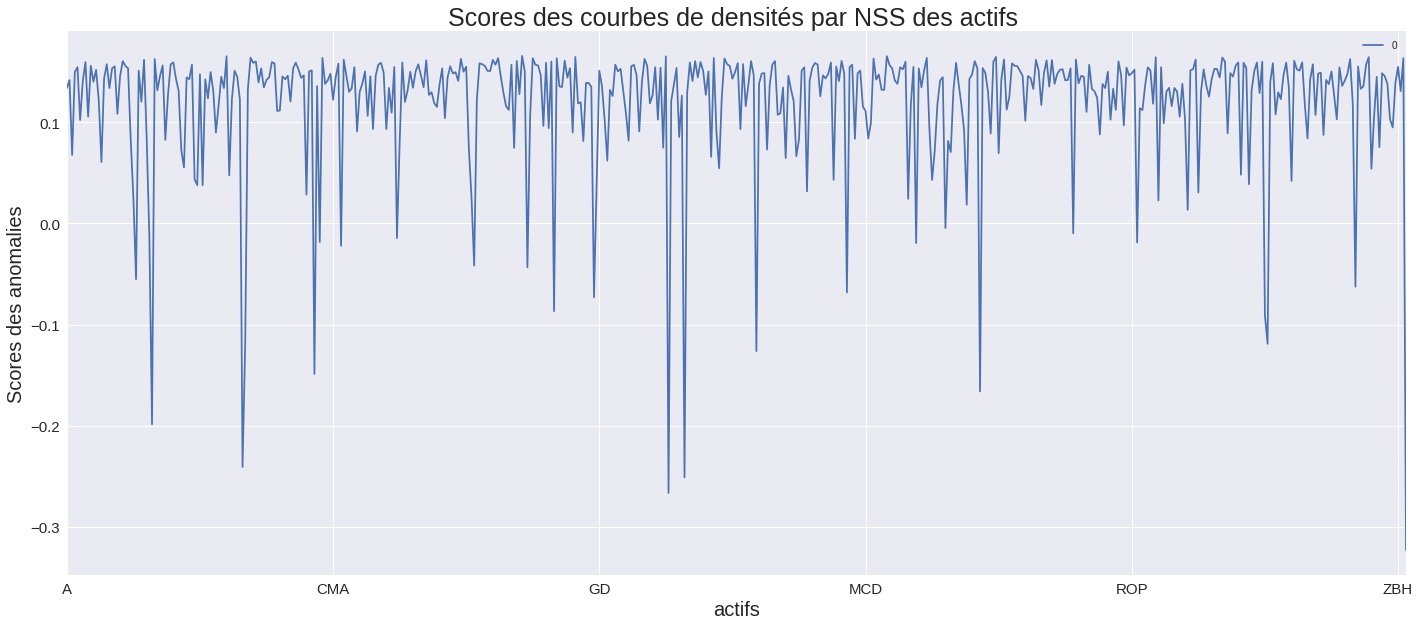
\includegraphics[scale=0.35]{img/scores_densite_nss_all.png}
 \label{anormm2}
\end{figure}

Score des anomalies isolées par la méthode de détection :

\begin{figure}[H]
\centering
\caption{Comparaison entre actifs "anormaux" et "normaux" (NSS)}
   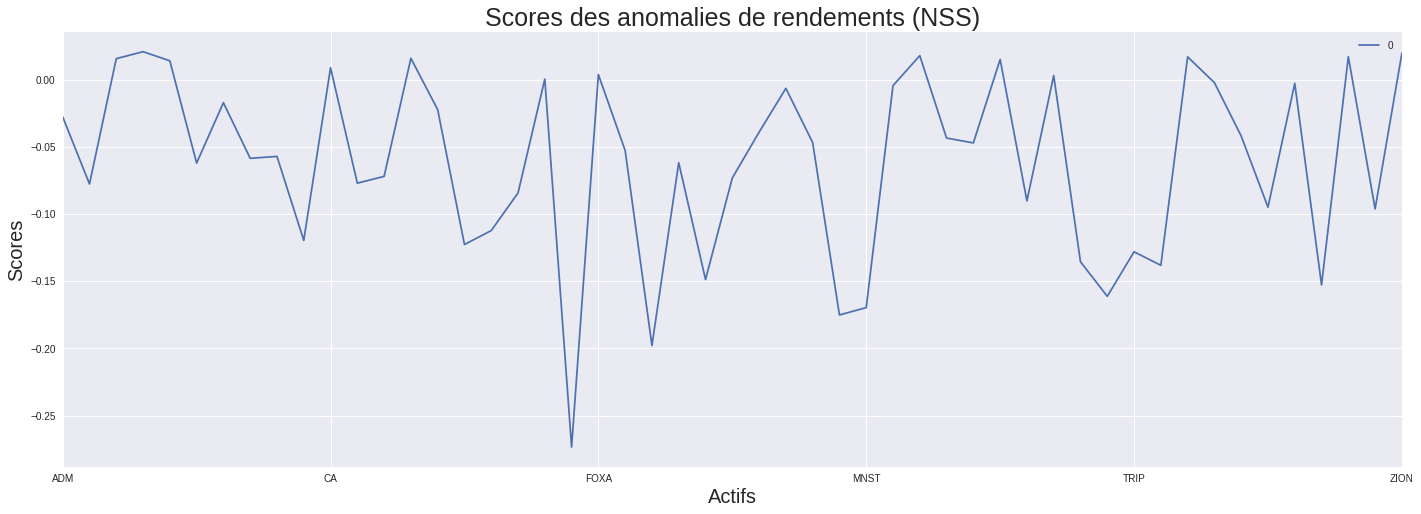
\includegraphics[scale=0.35]{img/scores_densite_NSS.png}
 \label{anormm1}
\end{figure}

Liste des actifs isolés :

['ADM', 'AFL', 'ALL', 'APC', 'APD', 'AVGO', 'BHF', 'BHGE', 'BK', 'BMY',
       'CA', 'CB', 'CHK', 'CME', 'CSX', 'DRE', 'DVN', 'ETN', 'EXC', 'FISV',
       'FOXA', 'GILD', 'GRMN', 'HLT', 'HPQ', 'JNJ', 'KSU', 'LB', 'LEG', 'M',
       'MDT', 'MNST', 'MRO', 'NOC', 'OKE', 'ORLY', 'PAYX', 'PFE', 'PSX', 'RRC',
       'SNA', 'TMO', 'TRIP', 'TROW', 'VTR', 'WMB', 'WMT', 'WYNN', 'XLNX',
       'ZBH', 'ZION']

Comparaison entre distributions normales en vert (A,ABBV) et anormales en rouge (ADM, ZION) sur la figure suivante:

\begin{figure}[H]
\centering
\caption{Comparaison entre actifs "anormales" et "normals" (NSS)}
   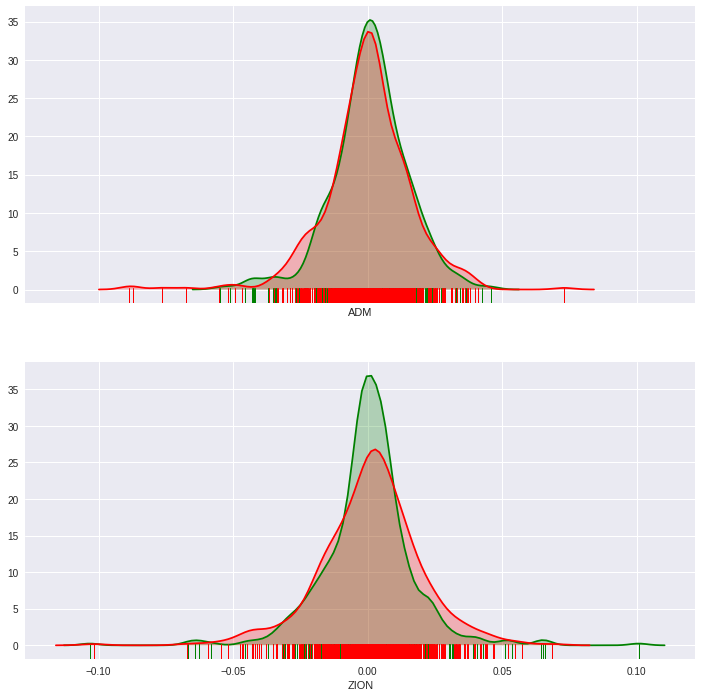
\includegraphics[scale=0.7]{img/anomalie_vs_normal_nss.png}
 \label{anormm}
\end{figure}

On peut bien noter les différences entre distribution normales et anormales soulignées par la méthode de détection par isolation. Cependant cette approche est à prendre avec prudence du faite de l'étape intermédiaire d'estimation non paramétrique des lois de probabilité des rendements.

%\subsection{Isolation des formes des courbes de distributions}

% system.time(sols <- lapply(df_den,solsf,de = de, OF=OF))
%utilisateur     système      écoulé 
%    6849.47        0.08     6851.69 

% part  (end)

\addcontentsline{toc}{chapter}{Conclusion}
\chapter*{Conclusion}

Python a été un véritable compagnon au cours de cette expérience professionnel. L'ensemble des missions ont été menées avec lui comme principal outil. Il se veut être une véritable alternanive, souple, puissant et polyvalant, à Microsoft Excel et SAS.
\\
\\
L'ensemble des missions sur lesquelles j'ai travaillé m'ont appris le sens de l'organisation, de l'objectivité et de l'autonomie. Il est nécessaire de connaître son objectif et de veiller à ne pas s'en éloigner. Certaines missions sont plus difficiles que d'autres, et certaines peuvent identifier des faiblesses existantes. Le monde professionnel est fait de challenge continuel, il faut pas hésiter remettre ses méthodes en question de même que ses approches. Certaines missions peuvent mener à des impasses, toutefois contournable, mais avec un coût de chantier en temps et en travail, plus élevé que prévu. C'est aussi le monde professionnel, dans un sens mathématique on dira que tout n'est pas linéaire et continue.
\\
\\
La méthode de détection d'anomalie par isolation est une méthode qui comme énoncée, se veut nouvelle et innovante, elle se démarque des méthodes basée sur les distances par une approche essentiellement stochastique. De son application, on obtient des résultats plutôt réalistes et convaincant. En plus elle fait économiser sur les coûts de calcul de distance et de stockage de matrice de distance énormes. Cependant, penser qu'elle est parfaite serait utopique. Il est important de l'appliquer sur les bonnes variables pour avoir les bonnes réponses tout en tenant compte du fait qu'elle puisse passer à côté de certaines anomalies.

\chapter*{Annexes}

\section*{Code python de l'application de la méthode d'isolation}

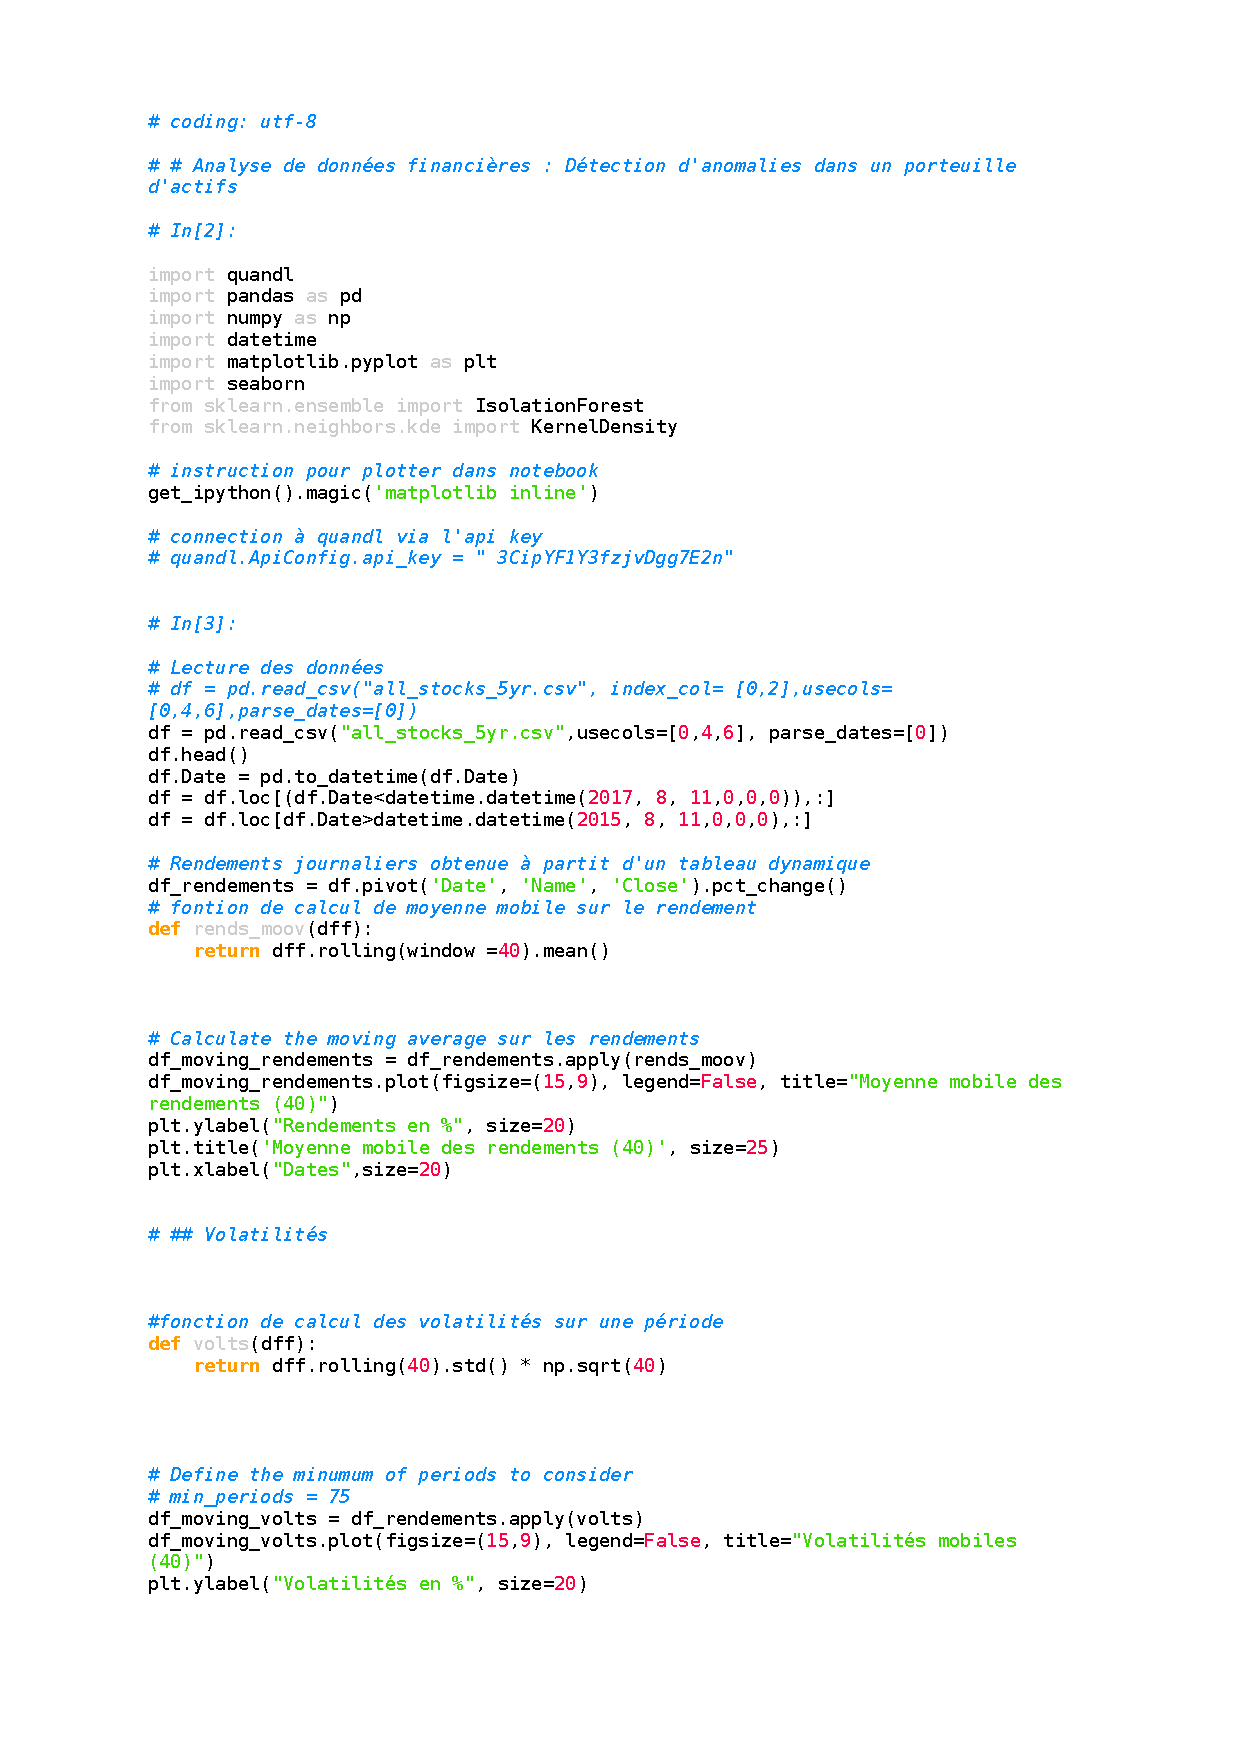
\includepdf[pages=-]{financial_data_1__py.pdf}

\section*{Code R de la calibration de Nielson-Siegel-Svensson}

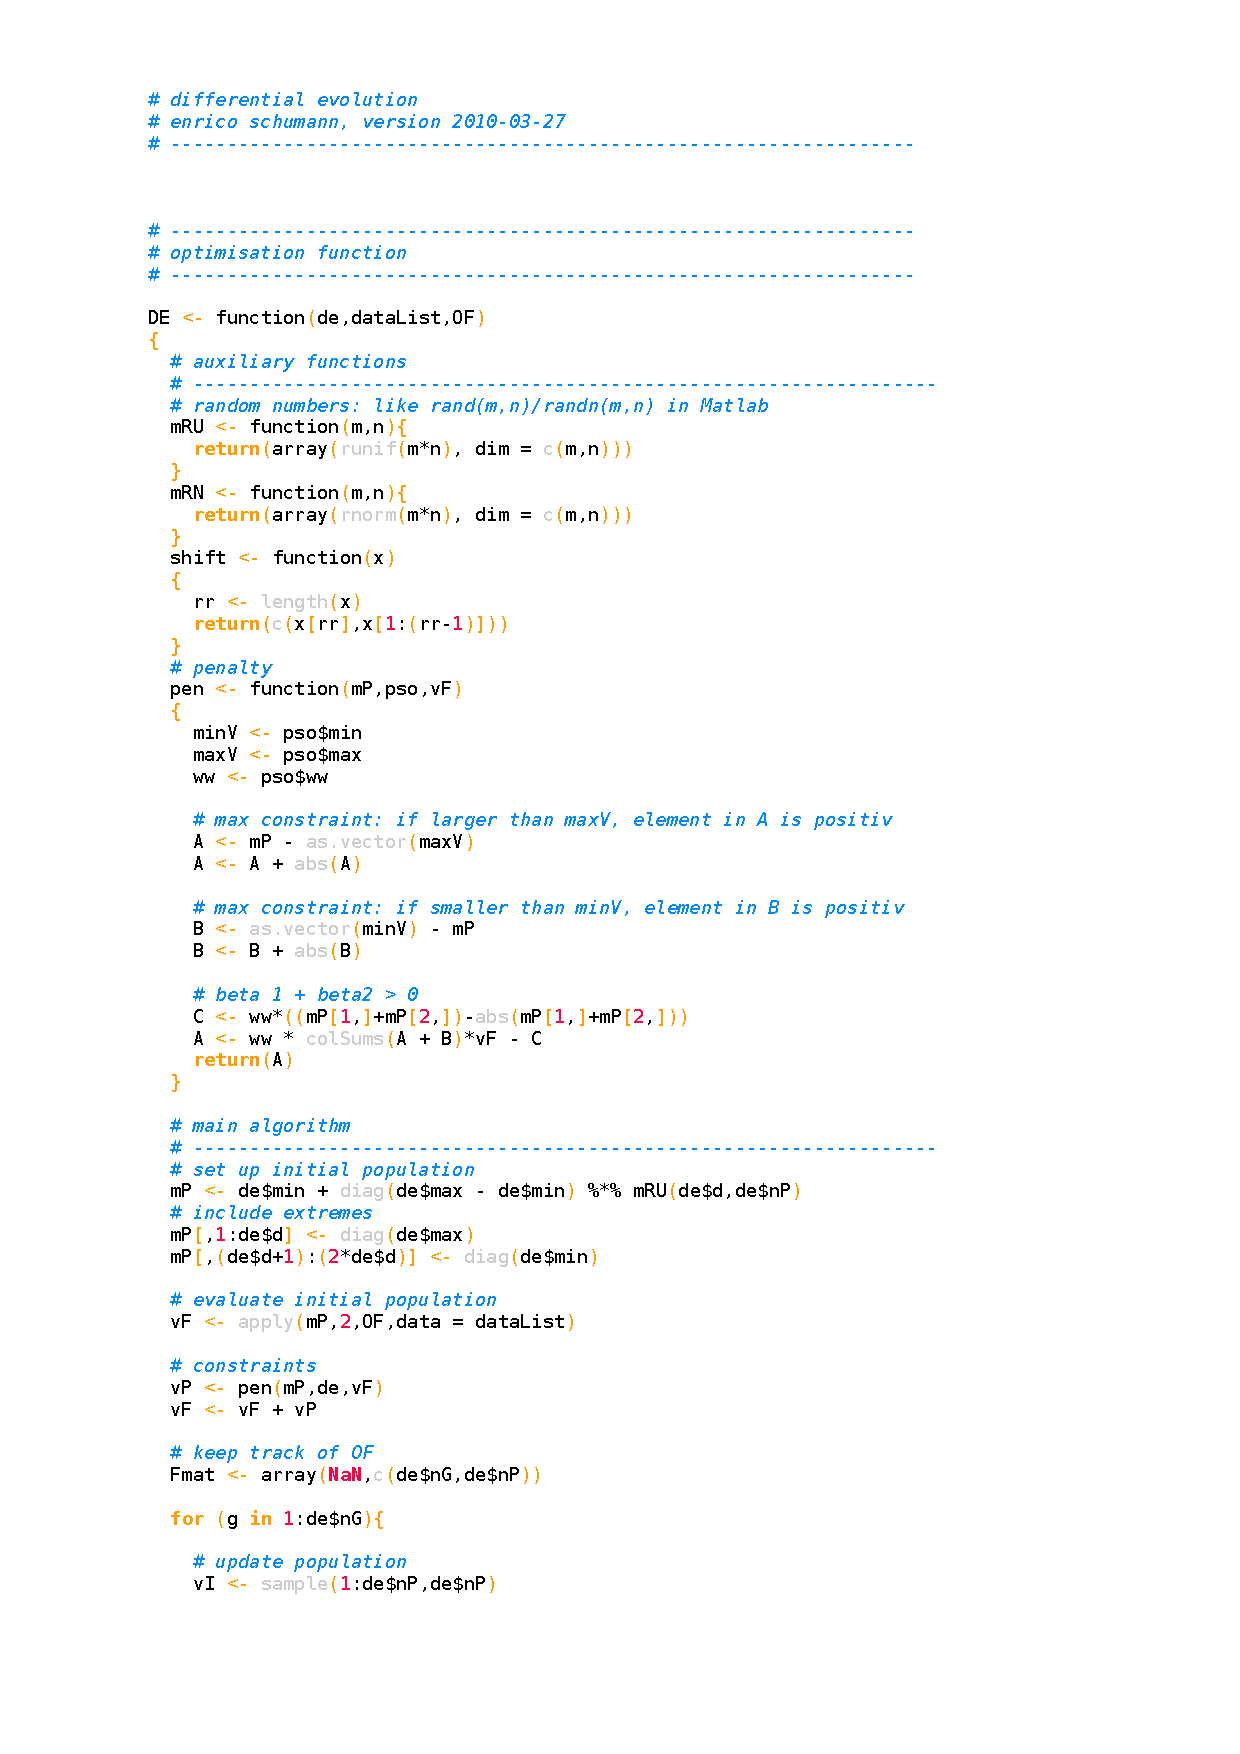
\includepdf[pages=-]{codes_R.pdf}

{\setlength{\baselineskip}{0.9\baselineskip}
\setcounter{tocdepth}{5} %defini la profondeur maximale des titres du sommaire
\tableofcontents % Sommire en debut et/ou table des matières en fin de rapport
\par}

\listoffigures

\listoftables

\bibliographystyle{plain}
\bibliography{biblio.bib}
\cite{Liu2012}
\cite{Hull2015}
\cite{STORN1997}
\cite{Befec-PriceWaterhouse1996}
\cite{ManfredGilli2010}
\\
\end{document}